%%%%%%%%%%%%%%%%%%%%%%%%%%%%%%%%%%%%%%%%%%%%%%%%%%%%%%%%%%%%%%%%%%%%%%%%%%%%%%%%%%%%%%%%%%%%%%%%%%%%%%%%%%%%%%%%%%%%%%%%%%%%%%%%%%%%%%%%%%%%%%%%%%%%%%%%%%%
% This is just an example/guide for you to refer to when submitting manuscripts to Frontiers, it is not mandatory to use Frontiers .cls files nor frontiers.tex  %
% This will only generate the Manuscript, the final article will be typeset by Frontiers after acceptance.   
%                                              %
%                                                                                                                                                         %
% When submitting your files, remember to upload this *tex file, the pdf generated with it, the *bib file (if bibliography is not within the *tex) and all the figures.
%%%%%%%%%%%%%%%%%%%%%%%%%%%%%%%%%%%%%%%%%%%%%%%%%%%%%%%%%%%%%%%%%%%%%%%%%%%%%%%%%%%%%%%%%%%%%%%%%%%%%%%%%%%%%%%%%%%%%%%%%%%%%%%%%%%%%%%%%%%%%%%%%%%%%%%%%%%

%%% Version 3.4 Generated 2022/06/14 %%%
%%% You will need to have the following packages installed: datetime, fmtcount, etoolbox, fcprefix, which are normally inlcuded in WinEdt. %%%
%%% In http://www.ctan.org/ you can find the packages and how to install them, if necessary. %%%
%%%  NB logo1.jpg is required in the path in order to correctly compile front page header %%%

\documentclass[utf8]{FrontiersinHarvard} % for articles in journals using the Harvard Referencing Style (Author-Date), for Frontiers Reference Styles by Journal: https://zendesk.frontiersin.org/hc/en-us/articles/360017860337-Frontiers-Reference-Styles-by-Journal
%\documentclass[utf8]{FrontiersinVancouver} % for articles in journals using the Vancouver Reference Style (Numbered), for Frontiers Reference Styles by Journal: https://zendesk.frontiersin.org/hc/en-us/articles/360017860337-Frontiers-Reference-Styles-by-Journal
%\documentclass[utf8]{frontiersinFPHY_FAMS} % Vancouver Reference Style (Numbered) for articles in the journals "Frontiers in Physics" and "Frontiers in Applied Mathematics and Statistics" 

%\setcitestyle{square} % for articles in the journals "Frontiers in Physics" and "Frontiers in Applied Mathematics and Statistics" 
\usepackage{url,hyperref,lineno,microtype,subcaption}
\usepackage{svg}
\usepackage[onehalfspacing]{setspace}
\usepackage{listings}
\usepackage{rotating}
\usepackage{tabularx}
\usepackage[english]{babel}
\usepackage{booktabs}
\usepackage{longtable}
\usepackage{multirow}
\usepackage{graphicx}
\usepackage[11pt]{moresize}
\newcommand{\TODO}[1]{{\color{red}{#1}}}

\lstset{
  basicstyle=\ttfamily,
  breaklines=true,  % Enable line breaking
  postbreak=\mbox{$\hookrightarrow$}  % Symbol for breakline
}

\lstdefinestyle{BashInputStyle}{
  language=bash,
  basicstyle=\small\sffamily,
  numbers=left,
  numberstyle=\tiny,
  numbersep=5pt,
  frame=single,
  columns=fullflexible,
  backgroundcolor=\color{lightgray},
  linewidth=\linewidth,
  xleftmargin=0.075\linewidth,
  literate={-}{-}1 {'}{{\textquotesingle}}1,
}

\linenumbers

% Leave a blank line between paragraphs instead of using \\

\def\keyFont{\fontsize{8}{11}\helveticabold }
\def\firstAuthorLast{Weaver {et~al.}} %use et al only if is more than 1 author
\def\Authors{Steven Weaver\,$^{1*}$, Vanessa Davila Conn\,$^{2}$, Daniel Ji\,$^{3}$, Hannah Verdonk\,$^{1}$, Joel O. Wertheim\,$^{3}$, and Sergei L. Kosakovsky Pond\,$^{1}$}
% Affiliations should be keyed to the author's name with superscript numbers and be listed as follows: Laboratory, Institute, Department, Organization, City, State abbreviation (USA, Canada, Australia), and Country (without detailed address information such as city zip codes or street names).
% If one of the authors has a change of address, list the new address below the correspondence details using a superscript symbol and use the same symbol to indicate the author in the author list.
\def\Address{$^{1}$ Center for Viral Evolution, Temple University, Philadelphia, PA, USA \\
$^{2}$ Center for Research in Infectious Diseases, National Institute of Respiratory Diseases, Mexico City, Mexico  \\ 
$^{3}$ Department of Medicine, University of California San Diego, La Jolla, CA, USA
}
% The Corresponding Author should be marked with an asterisk
% Provide the exact contact address (this time including street name and city zip code) and email of the corresponding author
\def\corrAuthor{Sergei L Kosakovsky Pond}

\def\corrEmail{spond@temple.edu}

\begin{document}
\onecolumn
\firstpage{1}

\title { AUTO-TUNE: SELECTING THE DISTANCE THRESHOLD FOR INFERRING HIV TRANSMISSION CLUSTERS }

\author[\firstAuthorLast ]{\Authors} %This field will be automatically populated
\address{} %This field will be automatically populated
\correspondance{} %This field will be automatically populated

\extraAuth{}% If there are more than 1 corresponding author, comment this line and uncomment the next one.
%\extraAuth{corresponding Author2 \\ Laboratory X2, Institute X2, Department X2, Organization X2, Street X2, City X2 , State XX2 (only USA, Canada and Australia), Zip Code2, X2 Country X2, email2@uni2.edu}

\maketitle

\begin{abstract}

	%%% Leave the Abstract empty if your article does not require one, please see the Summary Table for full details.
	\section{}

	\noindent Molecular surveillance of viral pathogens and inference of
	transmission networks from genomic data play an increasingly
	important role in public health 
	efforts, especially for HIV-1. For many methods, the genetic distance
	threshold used to connect sequences in the transmission network is a key
	parameter informing the properties of inferred networks. Using a distance
	threshold that is too high can result in a network with many spurious links,
	making it difficult to interpret. Conversely, a
	distance threshold that is too low can result in a network with too few links,
	which may not capture key insights into clusters of public health concern. Published research using the HIV-TRACE software package
	frequently uses the default threshold of $0.015$ substitutions/site for HIV pol gene sequences,
	but in many cases, investigators heuristically select other threshold parameters
	to better capture the underlying dynamics of the epidemic they are studying.

  Here, we present a general heuristic scoring approach for tuning a distance
  threshold adaptively, which seeks to prevent the formation of giant clusters.
  We prioritize the ratio of the sizes of the largest and the second largest
  cluster, maximizing the number of clusters present in the network.

  We apply our scoring heuristic to outbreaks with different characteristics,
  such as regional or temporal variability, and demonstrate the utility of
  using the scoring mechanism's suggested distance threshold to identify
  clusters exhibiting risk factors that would have otherwise been more
  difficult to identify. For example, while we found that a $0.015$ substitutions/site distance
  threshold is typical for US-like epidemics, recent outbreaks like the
  CRF07\_BC subtype among men who have sex with men (MSM) in China have been
  found to have a lower optimal threshold of $0.005$ to better capture the
  transition from injected drug use (IDU) to MSM as the primary risk factor.
  Alternatively, in communities surrounding Lake Victoria in Uganda, where
  there has been sustained heterosexual transmission for many years, we found
  that a larger distance threshold is necessary to capture a more risk
  factor-diverse population with sparse sampling over a longer period of time.
  Such identification may allow for more informed intervention action by
  respective public health officials.

	\tiny
	\keyFont{ \section{Keywords:} molecular epidemiology, HIV, network, transmission cluster, surveillance} %All article types: you may provide up to 8 keywords; at least 5 are mandatory.

\end{abstract}

\section{Introduction}

The use of genomic data to infer and characterize transmission networks of
various pathogens has grown in prominence in the past two decades, with
applications to a growing list of pathogens, including viruses such as HIV
\citep{paraskevis_application_2016}, hepatitis C virus (HCV)
\citep{murphy_molecular_2019}, or influenza A virus
\citep{jombart_reconstructing_2011}, and bacteria such as $M. tuberculosis$
\citep{mai_mycobacterium_2018} or $A. baumanii$ \citep{thoma_challenge_2022}.
Notably, genomic surveillance had a prominent role during the COVID-19
pandemic, including the use of sequencing for the study of transmission
clusters \citep{von_rotz_systematic_2023,campigotto_utility_2023}. Choosing an
appropriate genetic distance threshold is an important part of using a
molecular transmission network to track the spread of rapidly evolving
pathogens \citep{liu_dynamics_2020,rose_persistence_2020}. This distance
threshold defines the degree of genetic closeness between pathogen sequences,
isolated from two individuals, required to suggest them as potential
transmission partners in the network. Using a distance threshold that is too
large can result in a network with many spurious, making it difficult to
interpret and analyze. On the other hand, using a distance threshold that is
too small can result in a network with too few links, underestimating
connections between individuals and making it difficult to accurately track the
spread of the disease \citep{gore_hiv_2022}.

To enhance the utility of inferred transmission networks, it is important to
carefully consider the appropriate distance threshold, $d$. This threshold may
vary depending on the specific disease and the context in which it is
spreading. For example, a highly contagious acute respiratory illness (e.g.,
SARS-CoV-2) may require a smaller $d$ than a less contagious chronic illness
that is primarily spread through direct contact (e.g., HIV-1)\TODO{SAR --
	Reference}. Viruses are more amenable to molecular studies compared to bacteria
due to their high genetic divergence and compact genomes. Given the relatively
high evolutionary rate of RNA viruses 
detectable genetic fingerprints can be prioritized for epidemiological studies
over short time periods\citep{paraskevis_application_2016}.

For chronic infections such as HIV, the most appropriate genetic distance
threshold should be determined according to the characteristics of the epidemic
such as the speed of transmission, and the evolutionary rate of the genomic region
analyzed \citep{liu_dynamics_2020}. Sampling density and possible delays
between infection and diagnosis should be considered, since samples close to
the time of seroconversion are more likely to cluster than samples from well
after infection. Lower thresholds will capture the most closely related
sequences, while higher thresholds will capture long-term epidemics and
chronically infected individuals \citep{junqueira_factors_2019}.

Cluster analysis, i.e., identification and analysis of connected network
components, in public health has been used for early identification of
increased transmission \citep{oster_hiv_2021, oster_identifying_2018},
monitoring response to an HIV outbreak \citep{tumpney_human_2020,
sizemore_using_2020, tookes_rapid_2020}, evaluating the effectiveness of
interventions \citep{peters_hiv_2016,wang_targeting_2015,liu_dynamics_2020} or
predicting clusters that are most likely to grow in the near future
\citep{erly_predictive_2021,ragonnet-cronin_forecasting_2022}. This balance can
be achieved through careful analysis and consideration of the specific disease
and context.

This study introduces AUTO-TUNE, a method that offers a systematic approach to
select genetic distance thresholds for molecular HIV transmission network
analysis, based purely on the structure of the collected data. By autonomously
optimizing clustering metrics derived from pairwise genetic distances,
AUTO-TUNE has the potential to improve the accuracy and reliability of network
inference, irrespective of data attributes. The AUTO-TUNE methodology's
independence from supplementary data makes it less sensitive to variations in
data collection protocols and enhances its adaptability to various contexts,
including potentially other viral diseases.

\section{Methods}

Assume that there are $S$ aligned genomic sequences (full or partial, e.g. the
HIV-1 \textit{pol} gene) for a pathogen of interest, each representing the "consensus"
circulating viral diversity at the time of sampling in a single infected
individual. We shall infer a putative transmission network comprising $S$
nodes, and $E$ links (edges), where an edge is drawn between a pair of
sequences if the genetic distance between them is at or below a threshold $d$.
In such a network, there will be $0 \leq C < S$ connected components with more
than one node (clusters), which are the primary object of inference. This
network inference strategy is used by HIV-TRACE
\citep{kosakovsky_pond_hiv-trace_2018}, where the genetic distance is computed
using the Tamura-Nei (TN93) \citep{tamura_estimation_1993} model, with a
variety of options controlling how to deal with ambiguous nucleotide bases; for
HIV-1 such bases are informative since they often represent variants
co-circulating in the infected individual at the time of sampling at
substantial frequencies\TODO{SAR -- Reference}.

We begin by describing an approach to assign a score to each of the choices of
$d$ in a plausible/informative range of distances. Note that while such a range
is continuous, it is sufficient to only consider distance cutoffs that are in
the array of pairwise distances between the sequences, as those are the
cut-points where one or more additional edges will be added to the network as
$d$ is increased.

\subsection{Scoring Heuristic Procedure}

The network threshold selection procedure proceeds as follows (we provide an
example in the Results section as well).

\begin{enumerate}
	\item{For each candidate threshold $d_L$, in increasing order, ranging from the smallest genetic distance in the dataset, up to either the largest distance or a predetermined maximal threshold, we compute two network statistics: $R_{12}$, the ratio of the size of the largest cluster to the size of the second largest cluster, and $C$, the number of clusters in the network at this threshold. A cluster is defined as a connected component in the network with at least two nodes.}

	\item{ A priority score is assigned to each $d_L$. This score measures two properties of the threshold: Does $R_{12}$ jump at $d_L$? How far is the number of clusters $C$ at $d_L$ from the maximal number of clusters computed over all threshold values? Let there be $N$ overall $d_L$ candidate values, and assume we are examining the ith candidate, $d_L^i$ with $W < i \leq N - W$ ($W$ is a positive integer defined below).

	            \begin{enumerate}
		            \item{The $R_{12}$ jump is computed by looking at the normalized ratio of the mean $R_{12}$ values computed over the leading window $d_L^{i+1}…d_L^{i+W}$ and the trailing window $d_L^{i-W}… d_L^{i-1}$. The width of the window, $W$, is defined as $\min \left( \max \left(\left[\frac{N}{100}\right], 3\right), 30 \right)$. The distribution of ratios is converted to $Z$ scores, and normalized relative to the largest positive $Z$ score across all candidate distances, yielding the jump component of the score.}
		            \item{The number of clusters, $C_i$ at threshold $d_L^i$ is first normalized to $[0,1]$ through $\frac{{C_{max} - C_i}}{{C_{max} -C_{min}}}$ and next gated via a Gompertz function transform ${1-e}^{-e^{-25x+3}}$. This function provides an \emph{ad hoc} means for penalizing having too few clusters relative to the maximum over all ranges. For example, a threshold that yields $95\%$ of the maximal number of clusters receives a score of $0.996$,  a threshold that yields $85\%$ - a score of $0.376$, and a threshold that yields $60\%$ - a score of $0.0009$.}
		            \item{The priority score for $d_L^i$ is the sum of the two components defined in (a) and (b), and ranges from 0 to 2.}
	            \end{enumerate}}

	\item{The threshold with the highest priority score will be selected as the suggested automatic distance threshold, if the score is high enough ($1.9$ or more), and either of the two conditions hold.
	            \begin{enumerate}
		            \item{No other thresholds have priority scores of $1.9$ or higher}
		            \item{If other thresholds have priority scores of $1.9$ or higher, then the range of thresholds represented by these options is small (no more than $\log N$ times the mean step between successive $d_L^i$).}
	            \end{enumerate}}

	\item{If no single threshold can be selected in step 3, then the one with the highest priority score is suggested, and an inspection of a plot of scores is recommended to ensure that the threshold is sensible.}
\end{enumerate}

\subsection{Assortativity}

Degree-weighted homophily (DWH) is a measure of similarity between nodes in a
network based on their attributes (such as demographic characteristics or
behaviors) and their degree centrality (i.e., the number of connections they have to other
nodes in the network). It is used to quantify the extent to which nodes with
similar attributes tend to be connected to each other more frequently than
would be expected by chance\cite{RePEc:adr:anecst:y:2012:i:107-108:p:33-48}.
DWH is calculated as the ratio of the observed number of connections between
nodes with similar attributes to the expected number of connections between
such nodes, based on their network degree.

For any two subsets $A$ and $B$ of nodes in a network without singletons (each
node has a positive degree), define the weight between $A$ and $B$ as

\[
	W_{A,B} = \frac{1}{|A||B|} \sum_{i \in A, j\in B, (i,j) \text{are connected}} \frac{1}{d_i d_j},
\]

where $d_i$ is the degree of node $i$, and $|X|$ is the cardinality (size) of
subset $X$.

Then for any proper (not empty and not the complete network) subset of the
network, $G$, e.g. a group of nodes sharing an attribute, e.g., transmission
risk factor, define

\begin{equation}
	DWH = \frac{W_{G,G}+ W_{\bar G, \bar G} - 2W_{G,\bar G}}{|G|^{-2}\sum_{i\in G} 1 / d_i + |\bar G|^{-2}\sum_{i\in \bar G} 1 / d_i },
\end{equation}

with
\begin{itemize}
	\item{$\bar G$ : the complement of $G$ (all nodes not in $G$)}
	\item{$d_i$ : the degree of node $i$}
\end{itemize}

DWH ranges from $-1$ to $1$. A DWH value of $0$ indicates that there is no more
homophily than expected by chance (conditioned on network structure), while a
value of $1$ indicates that there is perfect homophily ($G$ consists of
connected components disconnected from the rest of the network). A value of
$-1$ is achieved for perfectly disassortative networks (the only links are
between $G$ and $\bar G$).

DWH has been used in social network analysis and in the study of how different
attributes are related to the formation of connections between
individuals\TODO{SAR -- Reference}. To assess whether or not DWH is
significantly different from $0$ (and from random expectation), we generate the
null distribution of DWH obtained by randomly reshuffling node attributes used
to define group $G$ and recomputing DWH for each such replicate.

\subsection{Implementation}

The software implementation involves a step-by-step process that utilizes the
HIV-TRACE suite of packages. It starts with calculating pairwise distances with
the {\tt tn93} tool and a supplied multiple sequence alignment. Thus generated
pairwise distances are supplied to the {\tt hivnetworkcsv} script while
providing the {\tt -A} keyword argument. A brief outline of the software's
implementation is as follows

\begin{enumerate}

	\item{ Calculate pairwise distances: The user first calculates the pairwise distances using the {\tt tn93} fast pairwise distance calculator, providing the maximum threshold value to consider ($0.03$ in this case, which may be revised upwards for sufficiently divergent sequences, as this provides an upper bound of thresholds to consider) and the input FASTA file. The command for this step is
	            \begin{lstlisting}[style=BashInputStyle]
 tn93 -t 0.030 -a resolve -g 0.05 pol.fasta > pairwise_distances.15.tn93.csv
\end{lstlisting}

	            Please note that the threshold should include the maximal range one is
	            intending to test.

	      }

	\item {Compute priority scores for each candidate threshold: The {\tt hivnetworkcsv} script is then executed with the required input file, format, and autotune option to generate a tab-separated output file, as shown below
	      \begin{lstlisting}[style=BashInputStyle]
 hivnetworkcsv -i pairwise_distances.15.tn93.csv -f plain -A 0 > autotune_report.tsv
\end{lstlisting}
	      }

	\item {Visualize the report: Users can upload the generated {\tt autotune\_report.tsv} file to \\
	      \url{http://autotune.datamonkey.org/analyze} for visualization and further analysis of the data. This web-based site extends the Datamonkey platform \citep{weaver_datamonkey_2018} to provide an interactive environment to explore scores and other metrics across the range of tested outputs. }

	\item {Run HIV-TRACE: Once AUTO-TUNEd threshold(s) are settled upon after review, the user runs the HIV-TRACE command with the appropriate input FASTA file, distance threshold, and other required arguments. The output is saved as a JSON file. An example command is
	      \begin{lstlisting}[style=BashInputStyle]
hivtrace -i ./INPUT.FASTA -a resolve -r HXB2_prrt -t < autotune_threshold > -m 500 -g .05 > hivtrace.results.json
	\end{lstlisting}
	      }

	      \subsubsection{Optional : Compute Assortativity Metrics}

	      \item{ Annotate results: The {\tt hivnetworkannotate} script is used to annotate the results obtained from the HIV-TRACE step with attributes. The script takes the JSON results file, node attributes file, schema file, and a resolve flag as input.
	                  \begin{lstlisting}[style=BashInputStyle]
hivnetworkannotate -n hivtrace.results.json -a node_attributes.json -g schema.json -r
	\end{lstlisting}
	                  For more information, users can refer to the {\tt hivnetworkannotate}
	                  documentation.\TODO{SAR -- Reference} }

	      \item{ Analyze the results with DWH: After the results file has been annotated, the user can proceed to the assortativity page, \url{http://autotune.datamonkey.org/assortativity}, for further analysis of the output. }

	      AUTO-TUNE is accessible on GitHub as part of the {\tt hivclustering} repository
	      (\url{https://github.com/veg/hivclustering})). It is integrated into the
	      command-line interface of the software as the {\tt -A} or {\tt --auto-profile}
	      argument. {\tt hivclustering} is a key component of the HIV-TRACE suite of
	      tools, a resource for the inference, analysis, and visualization of HIV
	      transmission networks.

	      The Degree Weighted Homophily (DWH) calculation tool was developed using {\tt
			      TypeScript}, a statically typed superset of {\tt JavaScript} that ensures
	      robustness and scalability. In an effort to promote accessibility and ease of
	      integration, the DWH tool is packaged and distributed through the Node Package
	      Manager (npm), enabling researchers and developers to conveniently incorporate
	      this advanced analytical tool into their own projects and workflows. DWH can be
	      used in-browser or as a command-line tool. Instructions for usage and
	      installation are found on Github (\url{https://github.com/veg/dwh}).

\end{enumerate}

The described workflow offers a systematic approach to analyze potential
distance thresholds for one's data with AUTO-TUNE, from calculating pairwise
distances to visualizing and annotating results.

\subsection{Visualization}

Visualizations of AUTO-TUNE results are accessible at
\url{http://autotune.datamonkey.org/analyze}. These include the priority score
plot, and the two contributing statistics: cluster count relative to the
maximum and the ratio of two largest cluster sizes. \ref{fig:webapp} An
assortativity tool is available at
\url{http://autotune.datamonkey.org/assortativity}, and is an analytical tool
engineered to facilitate the calculation of Degree Weighted Homophily (DWH)
values. It utilizes the DWH NPM package to generate a tabular representation of
DWH values corresponding to each value for a selected attribute annotation,
providing an exhaustive examination of the interrelationships for the field.
The tool also computes the panmictic (null) range, which involves a label
permutation test to generate the null distribution of DWH values. This feature
establishes a comparative baseline that aids in determining the significance of
homophily versus what would be expected by chance.

The visualization code is available on Github
(\url{https://github.com/stevenweaver/autotune-app/}).

\subsection{Comparisons with previously published analyses}

First, we set out to compare the thresholds used in numerous published studies
with those obtained by AUTO-TUNE. To select the data sets for this analysis, we
conducted a scientific literature search to identify studies focused on HIV
networks for public health purposes. We then filtered the studies that utilized
HIV-TRACE to infer genetic networks and had publicly available sequences. Due
to privacy concerns, HIV-1 sequences are frequently not released in the public
domain \cite{Inzaule:2023aa}.

We also attempted to include studies from different countries and regions,
enabling us to assess the performance of our method across various epidemic
contexts, risk groups, and network sizes in real-data sets that used variable
clustering thresholds.

Second, we compared AUTO-TUNE with the most direct published alternative: the
	{\tt clustuneR} method \citep{chato_public_2020}. We procured datasets from
\citep{wolf_short_2017} and \citep{vrancken_multi-faceted_2017} utilizing the
identical approach delineated in \cite{chato_public_2020}. These datasets,
namely Middle Tennessee, Seattle, and Alberta were processed using the workflow
described in Section 2.3. This enabled us to determine an optimal threshold for
each dataset using AUTO-TUNE. We further executed the command as detailed in
step 4 of Section 2.3, deploying thresholds previously established as optimal
by \citep{chato_public_2020}. Note that {\tt clustuneR} requires and uses
temporal information (dates sequences were collected), whereas AUTO-TUNE does
not.

Lastly, we evaluated the effect of sampling density on the genetic distance
threshold as determined by AUTO-TUNE, we implemented a strategy of random
subsampling from the original dataset sourced from \citep{rhee_national_2019}.
This study was selected due to its satisfactory AUTO-TUNE score when utilized
in its entirety, as well as its inherent design as a Geographically-Stratified
set of 716 \textit{pol} Subtype/CRF (GSPS) reference sequence dataset. The dataset,
which comprises 6034 samples gathered between 1989 and 2016, was subjected to
random subsampling ten times at proportions of $25\%$, $50\%$, and $75\%$ of
the original sample size. For each subsample, the optimal threshold and
associated scores were determined via AUTO-TUNE.

\section{Results}

\subsection{Comparisons with published HIV-1 molecular epidemiology studies}

We selected several publications citing HIV-TRACE for our analysis, primarily
because these studies not only referenced the tool but also made some or all of
their sequence data publicly available (Table~\ref{tab:paperComparison},
~\ref{tab:paperComparisonProp}). These studies adopted several different
approaches for selecting genetic distance thresholds, including using US CDC
guidelines \citep{yan_central_2020}, picking thresholds based on prior studies
\citep{sivay_hiv-1_2018}, and visually inspecting the numbers of clusters and
nodes in the networks across candidate distance thresholds
\citep{liu_dynamics_2020}. These thresholds, often qualitatively determined,
tended to be round numbers, and were usually determined using {\it ad hoc} or
subjective procedures. Some studies stratified their analyses by viral subtype
(major clade), while others did not (or this was not applicable).

A direct comparison with published networks is not feasible because only the
underlying sequence data (and often only some of the sequences) are made
available, not the networks themselves. To facilitate comparison here, we used
distance thresholds and all available sequences from primary publications to
infer transmission networks anew (the scripts for doing so and the
corresponding settings are available in \url{github.com/veg/auto-tune}) and
compare them with the networks obtained using the highest scoring AUTO-TUNE
threshold.

With a few exceptions (e.g \cite{dalai_combining_2018,sivay_hiv-1_2018}), both
the distance thresholds and the inferred networks were quite different, in
terms of the numbers of connected nodes, clusters, degree distributions, and
even hyper-parameters, such as the characteristic exponent of the scale free
degree distribution, $\rho$. This is true even for the studies where the
published threshold was tuned (typically to maximize the number of clusters).
AUTO-TUNE thresholds were larger than the published values in $13/21$ datasets,
and smaller in $8/21$ datasets.

\subsubsection{Examples of how changing thresholds affects inferred networks}

\paragraph{Cluster size reduction} The $0.02$ subs/site (substitutions/site)
threshold used by \citet{dalai_combining_2018} yielded one large cluster
composed of two loosely connected components (one PWID/HSX, one MSM, see Figure
2 in that paper). A minute change to the threshold by AUTO-TUNE to $0.0194\%$
splits one large cluster into three (some nodes also became disconnected),
separating the two major risk groups; this is because the "bridging"
connections were between these two thresholds (see Fig~\ref{fig:examples} panel
A). This minor change also reduced $R_{12}$ from $21$ to $2.6$.

\paragraph{Cluster size increase}  Increasing the $0.015\%$ subs/site threshold on data from \citet{Little:2014aa} combined
several small clusters (and singletons) into a single larger cluster, while
preserving the overall size and properties of the network (see
Fig~\ref{fig:examples} panel B). This change also reduced $R_{12}$ from $2.5$
to $1.5$.

\paragraph{Thinning out the network}  Reducing the $0.015\%$ subs/site threshold on data from \citet{rhee_national_2019}
dramatically reduced the size of the largest cluster, and thinned out most
clusters with five or more nodes (see Fig~\ref{fig:examples} panel C).

\paragraph{Materially changing the degree distribution of the network}  For the sequences from \citet{Li:2022aa}, AUTO-TUNE suggests $D = 1.483\%$ with
robust ($1.76$) confidence, whereas the original $D = 0.013$ subs/site was selected based
on maximizing the number of clusters (and likely rounding to the nearest
decimal). While the total number of the clusters only increases by $1$, the
number of nodes connected in the network grows from $95$ to $119$, and the
scale free exponent of the distribution is dramatically affected. The latter
is informed by the degree distribution of the network, and
Fig~\ref{fig:examples} panel D shows, the degree distribution is dramatically
affected. Many commonly used network-derived correlates (e.g. degree centrality) can
be strongly affected by such changes.

\paragraph{Expanding the network}  Increasing the $.015$ subs/site threshold in \citet{Billings:2019aa} to $2.33\%$ more
than doubles the number of nodes included (Fig~\ref{fig:examples} panel E)

Networks with high AUTO-TUNE scores are exemplified by the alignment (in the
distance space) of the points where the number of clusters is maximized and
where the network transitions to having an "unusually" large cluster (see
Fig.~\ref{fig:cases}, panel A). In cases of low scores, AUTO-TUNE effectively
falls back to maximizing the number of clusters as a function of the distance
thresholds, which is a common strategy found in empirical studies (see
Fig.~\ref{fig:cases}, panel B).

As expected, AUTO-TUNE inferred smaller thresholds for younger (e.g., studies
based in China) epidemics. While AUTO-TUNE will always return a score, in the
majority of cases there is no clear "winner" threshold, with priority scores
exceeding $1.5$ in only 6/18 cases (Table~\ref{tab:paperComparisonProp}). One
interpretation for such lack of clarity is that the underlying network has
several different (e.g. spatial, temporal, or subtype-specific) thresholds
which cannot be well-represented by any single value. For instance, when
analyzing the data from \citet{Yan:2021aa}, AUTO-TUNE returned a low score of
$1.14$ for $D=0.839\%$. However, when we split the data into major constituent
subtypes and ran AUTO-TUNE on each one separately, starkly discrepant
thresholds were found for different subtypes: $D=0.0102$ subs/site (score = $1.59$) for
CRF01, $D=0.00193$ subs/site (score = $2$) for CRF05, $D=0.02615$ subs/site (score = $1.65$) for B,
and $D=0.0111$ subs/site (score = $1.04$) for CRF07. Although many networks from the
literature tend to be dominated by sequences from the same subtype, in more
heterogeneous settings it seems prudent to partition the data by subtype
(corresponding to major phylogenetic clades), and perform network analyses
within subtypes.

\subsection{Comparisons with published non-HIV molecular epidemiology studies}

While HIV-1 epidemiology is the predominant niche for distance-based molecular
transmission analyses, other rapidly evolving viruses, especially HCV, have
also been analyzed with these approaches\citep{bartlett2017molecular}. Unlike HIV-1, there is considerably
less work on how to choose an appropriate distance threshold, further
complicated by the use of different genes to build networks (see
\citet{Chan:2020aa} for a comprehensive summary). Two commonly seen methods
exist: use some measure of intra-host variation (obtained by deep sequencing)
as a lower bound for the threshold, or tune $D$ to obtain some desired network
property, e.g., the maximal number of clusters. Like with HIV-1, we searched
the literature for relevant studies, and selected several with publicly
available sequence data.

Most of the datasets are much smaller and less systematically sampled than
those for HIV-1, and often combine highly divergent subtypes in the same
collection, making a joint analysis challenging. As with HIV-1, AUTO-TUNE
returns a wide range of scores and $D$ thresholds. For example, effectively
maximizing the number of clusters on rhinovirus sequences from
\citet{Ng:2022aa} yields a $D$ estimate very similar to that obtained by the
authors from intra-host variability -- information not available to AUTO-TUNE.
Table~\ref{tab:paperComparisonNotHIV}

\subsection{Large-scale HIV-1 database analyses}

\subsubsection{Markedly different thresholds for different subtypes}
Following the spirit of the analysis performed by \citet{Wertheim:2014aa}, we
downloaded partial {\it pol} sequences (between HXB-2 coordinates 2253 and
3200, one sequence per patient) from the Los Alamos HIV-1 Database, split them
by annotated subtype and applied AUTO-TUNE to individual subtypes with $1000$
or more sequences.

Some (but not all) HIV-1 subtypes often act as strong correlates of regional
and temporal distributions of sequences, and are expected to represent
epidemics with different sampling rates and transmission dynamics. These
differences are reflected in a wide range of mean pairwise distances and
inferred AUTO-TUNE thresholds shown in Table~\ref{tab:paperLANL}. For example,
the relatively young subtype A6, which is the most common subtype in the
countries of the former Soviet Union \cite{Abidi:2021aa}, has a low mean
pairwise distance ($0.046$) and a low AUTO-TUNE threshold ($0.0056$). In
contrast A1D recombinant sequences have high distance and threshold values
($0.089$ and $0.0323$, respectively), because sequences of this "subtype"
represent broadly circulating strains with complex backgrounds, and extensive
histories of recombination \cite{Foster:2014aa,Yebra:2015aa}.

There was extensive variability among subtypes in all high-level network
statistics, including the mean degree, fractions of nodes that were in the
network, and the characteristic exponent $\rho$, where $\rho$ is inferred from
by fitting the degree distribution to various network formation models, and
with $\text{Prob}(\text{degree} = k) \sim 1/k^\rho$ for large $k$.

For A1, B, C, and CRF08 networks there's very strong support for a single
AUTO-TUNE threshold (score $>1.9$), while for many other subtypes there is
extreme ambiguity in which threshold to choose (score $<1.1$). We suggest that
networks where AUTO-TUNE fails to find a single threshold may comprise
heterogeneous data which require multiple thresholds to resolve.

\subsubsection{Congruence of networks inferred from different genes}

Very few published studies of HIV-1 transmission networks use genes other than
	{\it pol}, and nearly all of the extrinsically motivated thresholds have been
derived for this gene, the utility of other genes and the appropriate $D$
values for them are unclear. Because of different rates of evolution in HIV-1
genes and, possibly, subtypes \cite{Penn:2008aa}, one would expect $D$ to be
different for different subtypes and genes. As a simple exercise, we downloaded
full-length HIV-1 genomes from the LANL database, stratified them by subtype,
and conducted AUTO-TUNE inference using four genomic segments: protease+reverse
transcriptase, integrase, matrix (gag), and the less variable gp41 segment of
the envelope gene.

Only three subtypes had $\geq 500$ full-length sequences in the LANL HIV
database (Table~\ref{tab:LANL:full}): B, C, and CRF01. As expected, the
inferred thresholds differed by gene and subtype, with lower thresholds
inferred for more slowly evolving segments (PR+RT and INT), and similar numbers
of clusters found in the resulting subtype-level networks. For all three
subtypes, the level of agreement between the four networks on whether or not
nodes were clustered or not (present / absent from the network), measured by
Krippendorff's $\alpha$ \cite{doi:10.1080/19312450709336664}, were
substantially higher than expected by chance ($\alpha = 0$). All four networks
also had between a quarter and a half of all the clusters in perfect agreement. 

\subsection{Evaluating Inferred Networks using Homophily}

Non-random mixing and attribute-based homophily are intrinsic characteristics
of human contact networks and can be expected to be present in transmission
networks, particularly in the context of HIV transmission. People frequently
engage in relationships with those who share similar attributes or behaviors,
such as risk factors (e.g., PWID, MSM). Recent evidence suggests that
race/ethnicity is also a strong predictor of homophily in HIV
networks\citep{ragonnet2021sorting}. The effect of these nonrandom mixing
patterns on the genetic diversity of HIV-1 has not only been extensively
explored via modeling and simulations \citep{goodreau_assessing_2006}, but the
structure of sexual contact networks has been found to directly influence
pathogen phylogenies \citep{robinson_how_2013}. Phylogenetic analysis of HIV
type 1 sequences has revealed distinct grouping patterns based on risk
behaviors \citep{holmes_molecular_1995}. The expectation of homophily is so
strong, that its disruption, e.g. the presence of a self-reported heterosexual
risk group individual in a cluster exclusively composed of MSMs has been used
as a marker of undisclosed/incomplete risk factor reporting
\cite{Ragonnet-Cronin:2018aa}. Therefore, when subject-level attributes are
available, homophily is an expected and desired feature of the network.

To assess the performance of an AUTO-TUNEd optimized threshold using
degree-weighted homophily, we first evaluated a CRF07\_BC network with national
survey data from China \cite{Ge:2021aa} . Each of the $8178$ pol sequences was
annotated with a transmission risk factor: heterosexual contact (Hetero),
people who use injection drugs (PWID), or men who have sex with men (MSM),
among other attributes.

When we analyze the dataset with AUTO-TUNE, local maxima of AUTO-TUNE scores
were achieved with $0.0076$ sub/site and $0.0019$ sub/site thresholds, at scores $1.137$ and $1.030$,
respectively. Notably, the DWH scores for PWID exhibited a significant surge at
these thresholds, indicating a robust pattern of increased PWID homophily even
when relatively low scoring. The close proximity of AUTO-TUNE scores and the
consistent rise in PWID homophily at $0.0076$ and $0.0019$ thresholds suggest
comparable performance at these thresholds compared to the default $0.015$
threshold, suggesting that these thresholds might be more effective in
representing homophilic relationships in this network. At each threshold—0.015,
0.0076, and 0.0019—all DWH scores for the risk groups (MSM, Hetero, and PWID)
lie outside their respective panmictic ranges. This consistently indicates
non-random mixing and attribute-based homophily across the network. Detailed
results are in Table~\ref{table:combined} and Table~\ref{table:panmictic}.

\TODO{VDC: it also makes sense epidemiologically that PWID (usually outbreaks) have lower scores (than 1.5\%) due to faster transmission or case identification, while aligning with the homophlilic pattern.}
\TODO{SW: VDC, do you have a reference for this?.}

\subsection{Comparison with clustuneR}

We benchmarked AUTO-TUNE versus {\tt clustuneR} \cite{chato_public_2020}, which
employs the recency of sample collection or diagnosis as individual-level
weights in a predictive model to estimate the growth of HIV clusters. The
thresholds deemed optimal by {\tt clustuneR} were found by a grid-search for
the minimum GAIC (generalized Akaike Information Criterion) across candidate
distances between $0$ and $0.04$ in steps of $8 \times 10^{-4}$. GAIC is the
difference between a null model that is only influenced by cluster size, and a
weighted model that includes individual-level attributes among known cases in
the cluster. Using the minimum GAIC metric, it was found that $0.016 (\pm
	0.5\times 10^{-4})$ was the optimal threshold for Tennessee and Seattle, and
$0.0104$ for Northern Alberta.

In contrast, AUTO-TUNE does not incorporate any attribute data in its scoring
heuristic. Instead, it relies on clustering metrics constructed purely from
pairwise distances between sequences. Using nearly same datasets analyzed by
	{\tt clustuneR} \citep{chato_public_2020}, AUTO-TUNE found the thresholds with
the highest scores to be $0.01872$ for Middle Tennessee, $0.01538$ for Seattle,
and $0.01201$ for Northern Alberta. \autoref{tab:homophily}. We use the
adjective "nearly" because we were not able to exactly match the number of
sequences analyzed in \citet{chato_public_2020} by obtaining the referenced
GenBank accession number and our best-effort intepretation of the filtering
steps.

Both methods agree that there is a qualitative relationship of $\text{Northern
		Alberta} < \text{Seattle} ~\sim \text{Tennessee}$ for distance thresholds.
AUTO-TUNE thresholds, while not optimal in the GAIC sense all yield
improvements over the null model, hence they are qualitatively similar to {\tt
		clustuneR} (Figure 4 in \cite{chato_public_2020}). AUTO-TUNE is notably faster
in computation than clustuneR due to the fact that AUTO-TUNE only clusters
based on pairwise distances rather than inferring a maximum-likelihood
phylogeny. For example, the entire pipeline for the Seattle dataset took less
than $16$ seconds on an Apple M1 Max. Alternatively, the tree inference step
alone with {\tt clustuneR} takes several hours to complete.

Because the methods optimize very different objectives and {\tt clustuneR}
makes use of additional data, broad agreement between the inferred thresholds
is encouraging.

\subsection{The Effect of Subsampling on Optimal Thresholds and AUTO-TUNE Scores}

To address the challenges of applying network inference algorithms to
incompletely sampled datasets, this study includes a focused evaluation of
AUTO-TUNE's performance across varying data densities. Given logistical
limitations, obtaining a fully sampled HIV transmission network is often
infeasible. Therefore, we label a dataset as 'full' to serve as a closest
approximation of a fully sampled network. Using the selected dataset as a
benchmark, we assess AUTO-TUNE's adaptability and robustness when applied to
sparser datasets, a prevalent issue in real-world settings.

Since the \citep{rhee_national_2019} dataset exhibited a clear optimal peak, we
used the dataset for analysis, and randomly sampled $10$ times from the entire
dataset at $25\%$, $50\%$, and $75\%$ each. The original full dataset
confidently determined $0.01699$ (AUTO-TUNE score $1.9998$).

Sampling at $25\%$ yielded a mean top threshold of $0.021509$, median at
$0.019765$, and standard deviation of $0.004388$ \ref{fig:subsampling}. $50\%$
yielded $0.018581$ and $0.01871$ mean and median, respectively with a standard
deviation of $0.001629$. Finally, $75\%$ calculated mean is approximately
$0.017403$, with a median of approximately $0.01699$. The standard deviation
was $0.000924$.

As the dataset becomes sparser due to subsampling, the algorithm tends to
select higher distance thresholds. This phenomenon can be understood by
considering the effect of reduced sampling density on the network topology.
Sparse datasets naturally result in less interconnected clusters. To capture a
comparable level of network connectivity as in denser datasets, higher distance
thresholds are necessary. This is evidenced by the observed mean thresholds:
\(0.021509\) at \(25\%\), \(0.018581\) at \(50\%\), and \(0.017403\) at
\(75\%\). The standard deviations also narrow as the sampling density
increases, corroborating the increased precision of the threshold selection in
denser datasets.

As the proportion increased from $25\%$ to $50\%$ and $75\%$, observable shifts
were also noted in the mean, median, and standard deviation of the AUTO-TUNE
scores. At $25\%$, the mean and median scores were $1.5585$ and $1.5014$
respectively, with a standard deviation of $0.3568$. At $50\%$, both mean and
median scores significantly increased to $1.8171$ and $1.9191$ respectively,
and the standard deviation dropped to $0.2482$. Upon reaching an AUTO-TUNE of
$75\%$, the mean and median scores rose further to $1.9870$ and $1.9997$
respectively, while the standard deviation shrank substantially to $0.0364$,
indicating higher consistency in scores.

Next to determine how well subsampled datasets aligned with the full dataset,
we used two primary outcomes to gauge this concordance: the proportion of nodes
that remained clustered after subsampling and the proportion of singletons from
the original network that clustered in the subsampled networks.

We observed a consistent increase in the proportion of nodes that remained
clustered from the 0.015 sub/site threshold to the AUTO-TUNE threshold for each
respective subsampling proportion, with 25\% subsampling being the most
profound difference rising from a roughly 80\%-86\% interquartile range (IQR)
for 0.015 threshold to a ~90\%~96\% IQR for AUTO-TUNE, which indicates that the
AUTO-TUNE thresholds retain a higher degree of stability in the network's
structure across sampling density (Please see Figure~\ref{fig:subsampling2},
Panel A).

Since the thresholds inferred by AUTO-TUNE for the subsampled networks were
larger than the "fully" sampled network, we also measured the impact of
thresholding on the network's nodes that were originally singletons. Across all
variations in subsampling rates, the proportion of sampled singletons that
clustered all maintained low IQRs (See Figure~\ref{fig:subsampling2}, Panel B).
This implies that while AUTO-TUNE is effective in maintaining the core
structure of the network, it does not significantly alter the clustering of
nodes that were singletons in the full dataset.

As the sample proportion increased, an upward trend was noted in average
AUTO-TUNE scores. Additionally, the standard deviation reduced significantly
when increasing sample proportion. This implies that as sampling becomes
denser, AUTO-TUNE will become more confident in determining the optimal
threshold for a particular dataset.

\section{Discussion}

AUTO-TUNE addresses the challenge of selecting an appropriate genetic distance
threshold to construct HIV transmission networks by implementing a heuristic
scoring system. This system is predicated on two key features of networks
generated by candidate genetic distance thresholds: a high number of clusters
and the absence of a giant component. Few small clusters indicate an
excessively low threshold, while a giant cluster comprising numerous sequences
signals an overly high threshold. The efficacy of AUTO-TUNE is evidenced by its
ability to select thresholds that yield higher quality clustering, as
demonstrated by improved Degree-Weighted Homophily (DWH) scores across various
datasets, epidemic contexts, and risk groups. Furthermore, AUTO-TUNE thresholds
not only matched but often outperformed those manually selected in prior
studies, thus underlining the benefits of a more systematic, automated, and
data-responsive approach.

For example, the results of our study suggest that AUTO-TUNE, which relies
solely on clustering metrics from pairwise distances, could be an effective
alternative to other distance-based methods, such as {\tt clustuneR} while less
time-consuming and possessing a gentle learning curve, which makes it easy to
use by personnel not specialized in bioinformatics and computer science.
Furthermore, the simplicity of the method without compromising results
represents an advantage over phylogenetic methods where, in addition to the
calculation of genetic distances, it must also determine a support/distance
threshold where a rationale for the selection of these thresholds is rarely
provided \citep{junqueira_factors_2019}.

AUTO-TUNE generated thresholds for all three examined datasets (Middle
Tennessee, Seattle, and Northern Alberta) that outperformed {\tt clustuneR}
using DWH on 3-year collection date windows across all three datasets. This
indicates that even without incorporating attribute data, AUTO-TUNE's scoring
heuristic could provide reliable thresholds for HIV clusters. However, for the
determination of the optimal genetic distance threshold, time-related and
context-specific factors might need to be considered if there is no significant
score for any one candidate threshold, especially if there are multiple peaks.
For example, during HIV outbreaks in injection drug users (that usually occur
over several months), it may be more appropriate to use the shorter genetic
distance threshold \citep{peters_hiv_2016,campbell_detailed_2017} between
multiple high-scoring thresholds. On the contrary, larger and more extended
epidemics over time exhibit a tendency toward larger genetic distance
thresholds in order to capture transmission than younger epidemics and less
densely sampled epidemic investigations
\citep{patil_exploring_2022,leung_molecular_2019,di_giallonardo_subtype-specific_2021}.

Our evaluation of publications citing HIV-TRACE revealed the largely
qualitative determination of distance thresholds. This approach may result in
less accurate or suboptimal thresholds due to a lack of systematic analysis. In
contrast, AUTO-TUNE offers a more systematic and granular approach to threshold
selection, with our findings demonstrating that even minor adjustments to the
distance can drastically change the score. Therefore, using AUTO-TUNE could
potentially improve the quality of HIV clustering and transmission network
studies.

The Degree-Weighted Homophily (DWH) evaluation showed that AUTO-TUNE could
improve network quality based on specific attributes, such as risk factor,
which is an important part of HIV studies and informing prevention measures
\citep{potterat_risk_2002,fujimoto_methodological_2021}. For example, the use
of AUTO-TUNE resulted in an increased DWH among the MSM, Hetero, and PWID
groups when analyzing a CRF07\_BC network. Additionally, the results from the
Rhee et al. dataset also demonstrated AUTO-TUNE's ability to improve DWH
geographically, enhancing the network's ability to accurately reflect
transmission dynamics.

\TODO{SAR -- This may also be dependent of the epidemiological context. In some
	scenarios, risk factors may overlap, and thus, separating for example PWID and
	MSM networks would not make sense.}

Our analysis of AUTO-TUNE's performance on subsamples of a dataset revealed its
sensitivity to sample size. The results indicated a correlation between
increased sample size and higher average AUTO-TUNE scores, as well as lower
score variability. This suggests that denser sampling could enhance AUTO-TUNE's
ability to determine the optimal threshold for a dataset. Further studies might
be needed to establish the minimum sample size required for reliable threshold
determination.

\subsection{When a Score is Below 1.9}

In some cases, multiple scores at different thresholds could suggest the
presence of inherently different scales in the network. For instance, if a
network combines both global and local transmission patterns, AUTO-TUNE may
produce more than one high score, reflecting these different scales. This was
observed in a study on HIV-1 CRF07\_BC transmission networks in China, where
two distinct clusters, 07BC\_N and 07BC\_O, showed different transmission
routes and geographic concentrations \citep{ding_characterizing_2022}. Such
network complexities could mean that different thresholds might offer more
accurate insights into subpopulations or transmission dynamics.

The use of AUTO-TUNE, while offering a method for automated threshold
selection, may not always provide a single, decisive score that unambiguously
determines the optimal threshold. In certain situations, several candidate
thresholds may yield similar AUTO-TUNE scores, making it difficult to single
out one as the clear-cut 'optimal' threshold. \TODO{VDC -- when would it be
	more likely to have those scenarios? Is it with lower sampling densities,
	heterogeneous epidemics (e.g. multiple HIV subtypes or risk groups within the
	network)?} In these scenarios, the process of threshold selection becomes more
nuanced and requires a deeper analysis. The plot of AUTO-TUNE scores across
candidate thresholds can serve as a valuable tool in these cases. For instance,
researchers could identify a range of thresholds that all produce similar
scores, suggesting that the specific choice of threshold within this range may
not significantly impact the resulting network. Moreover, combining AUTO-TUNE
with the DWH measure can enhance the interpretation of such plots. By
considering how assortativity changes across the range of candidates,
researchers can make more informed decisions about the appropriate choice. If
there is a certain threshold at which the DWH measure noticeably changes for an
attribute of interest, this could suggest a meaningful shift in the network
structure that would be worth considering when selecting a threshold. The
symbiotic approach of combining AUTO-TUNE scores, DWH measure, and visual
analysis of score plots provides a more nuanced method for threshold selection
when no clear optimal threshold emerges from the AUTO-TUNE scores alone.

The AUTO-TUNE methodology has several limitations. First, even though it
provides the advantage of operating without the need for metadata, the size and
the subgenomic region analyzed may affect the accuracy of transmission
inference \citep{junqueira_factors_2019}. Second, our analysis of AUTO-TUNE's
performance on subsamples of a dataset revealed its sensitivity to sample size,
as the performance of the method can be affected by sampling density, improving
the reliability of the test as the sampling density increases (figure X).
However, our results were consistent with previous studies, which have
suggested an optimal sampling density of $50-70\%$ for HIV-1 cluster analysis
\citep{novitsky_impact_2014}. Third, even when it provides an insight of the
optimal threshold to analyze a network, the supplied information might still
need validation by experts, especially when no clear threshold is identified.
In this case, it has been recommended to combine genetic data with clinical and
sociodemographic information for a better characterization of the network
structure. Finally, the performance of the method needs to be assessed in
pathogens different from HIV, leading to opportunities for future research.

\section{Conclusion}

AUTO-TUNE operates solely utilizing genetic sequence data to ascertain a
decisive threshold. It employs a scoring heuristic, which is based on the
number of clusters produced by a pairwise distance threshold and the ratio of
the largest cluster to the second largest across a range of possible thresholds
using sliding windows.

A key advantage of this approach is its autonomy from supplementary data. When
a patient receives an HIV diagnosis, data collection protocols can greatly vary,
and additional data are not always available or consistent. However, by
leveraging only genetic sequence data, AUTO-TUNE eliminates the need for such
information in some cases, and at minimum serves as a preliminary assessment of
candidate thresholds.

Consequently, AUTO-TUNE's performance is consistently controlled, irrespective
of the fluctuations seen in data collection protocols after an HIV
diagnosis. This level of adaptability demonstrates its suitability for
integration into various contexts related to HIV, and possibly other viral
cluster detection and response protocols. This versatility underscores the
strong methodological foundation of AUTO-TUNE and its potential utility.

\section*{Conflict of Interest Statement}
%All financial, commercial or other relationships that might be perceived by the academic community as representing a potential conflict of interest must be disclosed. If no such relationship exists, authors will be asked to confirm the following statement: 

The authors declare that the research was conducted in the absence of any
commercial or financial relationships that could be construed as a potential
conflict of interest.

\section*{Author Contributions}

The Author Contributions section is mandatory for all articles, including
articles by sole authors. If an appropriate statement is not provided on
submission, a standard one will be inserted during the production process. The
Author Contributions statement must describe the contributions of individual
authors referred to by their initials and, in doing so, all authors agree to be
accountable for the content of the work. Please see
\href{https://www.frontiersin.org/guidelines/policies-and-publication-ethics#authorship-and-author-responsibilities}{here}
for full authorship criteria.

\section*{Funding}
SLKP and SW were supported in part by grant funding from the NIH, grants AI134384, AI140970, GM144468, and GM110749. JOW was supported in part by AI135992.

\section*{Acknowledgments}
This is a short text to acknowledge the contributions of specific colleagues, institutions, or agencies that aided the efforts of the authors.

\section*{Supplemental Data}
\href{https://www.frontiersin.org/guidelines/author-guidelines#supplementary-material}{Supplementary Material} should be uploaded separately on submission, if there are Supplementary Figures, please include the caption in the same file as the figure. LaTeX Supplementary Material templates can be found in the Frontiers LaTeX folder.

\section*{Data Availability Statement}

No new data were generated by our studies.

\bibliographystyle{Frontiers-Harvard} %  Many Frontiers journals use the Harvard referencing system (Author-date), to find the style and resources for the journal you are submitting to: https://zendesk.frontiersin.org/hc/en-us/articles/360017860337-Frontiers-Reference-Styles-by-Journal. For Humanities and Social Sciences articles please include page numbers in the in-text citations 
%\bibliographystyle{Frontiers-Vancouver} % Many Frontiers journals use the numbered referencing system, to find the style and resources for the journal you are submitting to: https://zendesk.frontiersin.org/hc/en-us/articles/360017860337-Frontiers-Reference-Styles-by-Journal
\bibliography{references}
\nocite{*}

%%% Make sure to upload the bib file along with the tex file and PDF
%%% Please see the test.bib file for some examples of references

\clearpage

\section*{Tables}

\begin{table}[h!]
	\caption{Comparison of AUTO-TUNE and published thresholds from prior studies using partial HIV-1 polymerase gene sequences. $N$ : the number of sequences; $L$: length of the multiple sequence alignment, bp; $E[D]$ mean pairwise TN93 distance; (the studies are sorted on this column, in ascending order) $\P$: the original study performed threshold tuning (varied methods); $\dagger$ : distance thresholds were specific to subtypes; $\star$ : the corresponding AUTO-TUNE score is $\geq 1.9$; $\bullet$ : only a subset of the complete dataset was made available (privacy, data use restrictions, incomplete GenBank submissions), the number of  sequences analyzed here is shown after the / symbol; N.R: not reported}
	\label{tab:paperComparison}

	\vspace{10pt}
	\centering
	\begin{ssmall}
		\begin{tabular}{llllllllll}
			\hline
			Reference                   & $N$                 & $L$  & $E[D]$ & Scope      & Location/Country         & Timespan  & Common                & \multicolumn{2}{c}{Distance threshold, sub/site}                  \\
			                            &                     &      &        &            &                          &           & Subtypes              & Published                                  & AUTO-TUNE      \\
			\hline
			\cite{Zai:2020aa}           & 209                 & 1056 & 1.5\%  & Country    & China                    & 2007–2015 & CRF55/01B             & $\P$ 0.002                                   & 0.00255          \\
			\cite{liu_dynamics_2020}    & 2087/1907 $\bullet$ & 1053 & 5.3\%  & City       & Shenyang, China          & 2008-2016 & CRF01, CRF07, B       & $\P$ 0.005/0.007 $\dagger$                     & 0.00621          \\
			\cite{dalai_combining_2018} & 317                 & 1044 & 5.5\%  & City       & San Mateo, CA, USA       & 1997-2008 & $96\%$ B              & 0.02                                          & 0.01944          \\
			\cite{chato_public_2020}    & 808                 & 1017 & 5.6\%  & Province   & Northern Alberta, Canada & 2007-2013 & B                     & $\P$0.0104                                   & 0.01201          \\
			\cite{Little:2014aa}        & 648/646 $\bullet$   & 1212 & 5.9\%  & City       & San Diego, CA, USA       & 1996-2011 & $98.5\%$ B            & 0.015                                        & 0.02495          \\
			\cite{Perez-Losada:2017aa}  & 1879/3411 $\bullet$ & 1027 & 6.0\%  & City       & Washington DC, USA       & 1987–2015 & B                     & 0.010                                        & 0.01733          \\
			\cite{rhee_national_2019}   & 4553                & 897  & 6.1\%  & State      & CA, USA                  & 1998-2016 & 95.5\% B              & 0.015                                        & 0.01139$\star$   \\
			\cite{chato_public_2020}    & 2779/2750 $\bullet$ & 1398 & 6.3\%  & State      & Tennessee, USA           & 2001-2015 & B                     & $\P$0.016                                    & 0.01872          \\
			\cite{Temereanca:2017aa}    & 37                  & 1302 & 6.7\%  & City       & Bucharest, Romania       & 2010-2013 & F1, G, B              & 0.015                                        & 0.00194          \\
			\cite{brenner_role_2021}    & 10945/448 $\bullet$ & 738  & 6.7\%  & Province   & Quebec, Canada           & 2002-2020 & B                     & 0.015/0.025\                                   & 0.02741          \\
			\citet{sivay_hiv-1_2018}    & 201                 & 1302 & 6.9\%  & Province   & Mpumalanga, South Africa & 2011-2015 & C                     & 0.025                                        & 0.02506          \\
			\cite{Li:2022aa}            & 295                 & 1206 & 7.8\%  & Prefecture & Pu'er, China             & 2021      & CRF08, CRF01, CRF07   & $\P$ 0.013                                   & 0.01483  $\star$ \\
			\cite{Yu:2022aa}            & 316                 & 1074 & 7.9\%  & Province   & Guangxi, China           & 2012-2018 & CRF01, CRF08, CRF07   & $\P$0.013                                    & 0.01178          \\
			\cite{Yan:2021aa}           & 1695/1569 $\bullet$ & 1569 & 8.4\%  & City       & Guangzhou, China         & 2008-2012 & CRF01, CRF07, CRF55,G & 0.015                                        & 0.00839          \\
			\cite{Billings:2019aa}      & 150                 & 1597 & 8.5\%  & City       & Lagos, Nigeria           & 2013-2016 & CRF02, URF            & 0.015                                        & 0.0233           \\
			\cite{Chen:2023aa}          & 1975/209  $\bullet$ & 1050 & 8.7\%  & Province   & Guangxi, China           & 2016-2018 & CRF01, CRF07, CRF08   & $\P$0.0075                                   & 0.01295          \\
			\cite{Fabeni:2020aa}        & 726/3499 $\bullet$  & 1029 & 9.2\%  & Country    & Italy                    & 1998-2018 & B                     & 0.010                                        & 0.0037           \\
			\cite{Leal:2020aa}          & 630/633 $\bullet$   & 990  & 9.2\%  & State      & Maranhão, Brazil         & 2008-2017 & B                     & 0.020                                        & 0.04033          \\
			\cite{bbosa_short_2020}     & 2018                & 1257 & 9.3\%  & Country    & Uganda                   & 2009-2016 & N.R                   & 0.015                                        & 0.02035 $\star$  \\
			\cite{Stecher:2018aa}       & 2774                & 1028 & 12.1\% & Multi-City & Germany                  & 1999-2016 & B                     & 0.015                                        & 0.03056          \\
			\cite{chato_public_2020}    & 1653/1840 $\bullet$ & 1020 & 5.5\%  & City       & Seattle, ISA             & 2000-2013 & B                     & $\P$0.016                                    & 0.01538          \\
			\\

			\hline
		\end{tabular}
	\end{ssmall}
\end{table}

\begin{table}[h!]
	\caption{Network properties at the published and AUTO-TUNE thresholds. In cases when the original paper used more than one threshold, we selected the largest for comparison. The datasets are ordered by the AUTO-TUNE priority score from highest to lowest. $\rho$ is the fitted characteristic scale-free exponent of the corresponding degree distributions.}
	\label{tab:paperComparisonProp}
	\vspace{10pt}
	\centering
	\begin{ssmall}
		\begin{tabular}{llllllllll}
			\hline
			Reference                        & AUTO-TUNE & \multicolumn{2}{c}{Nodes in network} & \multicolumn{2}{c}{Clusters in network} & \multicolumn{2}{c}{$R_{12}$} & \multicolumn{2}{c}{Scale parameter $\rho$}                                                 \\
			                                 & score     & Published                            & AUTO-TUNE                               & Published                    & AUTO-TUNE                                  & Published & AUTO-TUNE & Published & AUTO-TUNE \\
			\hline
			\cite{Li:2022aa}                 & 2.00      & 1364                                 & 1224                                    & 277                          & 277                                        & 1.7       & 2.4       & 2.8       & 2.6       \\
			\cite{chato_public_2020} TN      & 2.00      & 394                                  & 445                                     & 108                          & 109                                        & 1.0       & 1.7       & 2.7       & 2.9       \\
			\cite{rhee_national_2019}        & 1.95      & 2044                                 & 1636                                    & 524                          & 488                                        & 13.2      & 1.5       & 2.6       & 2.7       \\
			\cite{bbosa_short_2020}          & 1.93      & 222                                  & 296                                     & 102                          & 119                                        & 2.2       & 1.6       & 3.2       & 2.6       \\
			\citet{dalai_combining_2018}     & 1.89      & 60                                   & 54                                      & 9                            & 11                                         & 22        & 2.6       & 2.0       & 2.2       \\ % CONFIRMED
			\cite{Temereanca:2017aa}         & 1.79      & 30                                   & 16                                      & 5                            & 3                                          & 3         & 1.5       & N/A       & 2.8       \\
			\cite{Yu:2022aa}                 & 1.76      & 55                                   & 51                                      & 19                           & 19                                         & 2.75      & 1.75      & 10.4      & 34.0      \\
			\citet{sivay_hiv-1_2018}         & 1.42      & 51                                   & 51                                      & 19                           & 19                                         & 1.5       & 1.5       & 3.2       & 3.0       \\
			\cite{Zai:2020aa}                & 1.40      & 96                                   & 98                                      & 26                           & 27                                         & 1.5       & 1.5       & 24.1      & 17.7      \\ % CONFIRMED
			\cite{Little:2014aa}             & 1.31      & 301                                  & 394                                     & 98                           & 87                                         & 2.5       & 6.1       & 3.6       & 3.1       \\ % CONFIRMED
			\cite{brenner_role_2021}         & 1.22      & 363                                  & 379                                     & 71                           & 70                                         & 5.6       & 5.5       & 2.7       & 2.8       \\
			\cite{Stecher:2018aa}            & 1.20      & 97                                   & 558                                     & 36                           & 155                                        & 2.2       & 4.9       & 3.2       & 3.3       \\
			\cite{chato_public_2020} Seattle & 1.16      & 505                                  & 484                                     & 148                          & 149                                        & 2.5       & 1.7       & 2.7       & 2.6       \\
			\cite{Billings:2019aa}           & 1.16      & 38                                   & 78                                      & 13                           & 23                                         & 2         & 2.3       & 2.6       & 11.5      \\
			\cite{Yan:2021aa}                & 1.14      & 1084                                 & 753                                     & 124                          & 116                                        & 2.0       & 1.8       & 1.2       & 2.0       \\
			\cite{Chen:2023aa}               & 1.11      & 20                                   & 47                                      & 8                            & 16                                         & 1.3       & 2.0       & $\infty$  & $\infty$  \\
			\cite{Leal:2020aa}               & 1.11      & 50                                   & 270                                     & 25                           & 57                                         & 1         & 1.6       & 53.6      & 3.1       \\
			\cite{Perez-Losada:2017aa}       & 1.06      & 172                                  & 431                                     & 76                           & 134                                        & 5.1       & 1.4       & 5.2       & 2.9       \\
			\cite{liu_dynamics_2020}         & 1.05      & 885                                  & 797                                     & 156                          & 161                                        & 6.0       & 4.5       & 3.1       & 3.0       \\ % CONFIRMED
			\cite{chato_public_2020} Alberta & 1.03      & 394                                  & 445                                     & 108                          & 109                                        & 1.0       & 1.7       & 2.7       & 2.9       \\
			\cite{Fabeni:2020aa}             & 1.00      & 626                                  & 221                                     & 197                          & 83                                         & 2.1       & 3.2       & 2.1       & 3.2       \\

			\hline
		\end{tabular}
	\end{ssmall}
\end{table}

\begin{table}[h!]
	\caption{Comparison of AUTO-TUNE and published thresholds from prior studies using sequences from viruses other than HIV-1. "N/A": no distance-based clustering analyses were done. Other notation is the same as in Table~\ref{tab:paperComparison}}
	\label{tab:paperComparisonNotHIV}

	\vspace{10pt}
	\centering
	\begin{ssmall}
		\begin{tabular}{lllllllllll}
			\hline
			Reference               & Virus      & Gene          & $N$                & $L$        & $E[D]$                               & Scope    & Location/Country       & Timespan  & \multicolumn{2}{c}{Distance threshold, subs/site}                     \\
			                        &            &               &                    &            &                                      &          &                        &           & Published                                  & AUTO-TUNE (score) \\
			\hline
			\cite{Jia:2023aa}       & HCV        & {\it NS5B}    & 503                & 315        & 34.9\%                               & Province & Yunnan, China          & 2008–2018 & N/A                                        & 1.933 (1.92)      \\
			                        &            &               & 97                 & 8.0\%      & \multicolumn{4}{l}{Genotype 1b only} & $\P$ 2.3 & 1.944 (2.0)                                                                                         \\
			                        &            &               & 53                 & 7.4\%      & \multicolumn{4}{l}{Genotype 2a only} & $\P$ 3.3 & 3.3 (1.3)                                                                                           \\
			                        &            &               & 110                & 5.4\%      & \multicolumn{4}{l}{Genotype 3a only} & $\P$ 2.0 & 3.6 (1.0)                                                                                           \\
			                        &            &               & 189                & 5.5\%      & \multicolumn{4}{l}{Genotype 3b only} & $\P$ 1.7 & 1.6 (1.0)                                                                                           \\
			\cite{Murphy:2019aa}    & HCV        & {\it NS5B}    & 119                & 340-850    & 5.6\%                                & Province & Quebec, Canada         & 2001–2017 & N/A                                        & 0.0251 (1.05)     \\
			\cite{Paraschiv:2017aa} & HCV        & {\it NS5B}    & 117                & $\sim 300$ & 24.6\%                               & Country  & Romania                & 2011-2014 & N/A                                        & 1.394 (1.11)      \\
			\cite{Ye:2023aa}        & HCV        & {\it NS5B}    & 1603/399 $\bullet$ & 701        & 27.6\%                               & Country  & China                  & 1999-2017 & $\P$ 0.010                                   & 0.359 (1)         \\
			                        &            & {\it C/E2}    & 865/396 $\bullet$  & 837        & 37.3\%                               &          &                        &           & $\P$ 0.0325                                  & 1.572 (1.98)      \\
			\cite{Ng:2022aa}        & Rhinovirus & {\it VP2/VP4} & 977                & 388        & 43.2\%                               & City     & Kuala Lumpur, Malaysia & 2012-2014 & $\P$ 0.005                                   & 0.523 (1)         \\

			\hline
		\end{tabular}
	\end{ssmall}
\end{table}

\begin{table}[h!]
	\caption{An application of AUTO-TUNE to subtype stratified HIV-1 pol sequences from the LANL database. Fraction clustered is the proportion of all sequences that are connected to at least one other sequence. Subtypes are sorted by the inferred threshold, lowest first. Other notation is the same as in Table~\ref{tab:paperComparison}}
	\label{tab:paperLANL}

	\vspace{10pt}
	\centering
	\begin{small}
		\begin{tabular}{llllllll}
			\hline
			Subtype                        & $N$   & $E[D]$ & \multicolumn{2}{c}{AUTO-TUNE} & Fraction & Mean          & $\rho$        \\
			                               &       &        & Threshold, \%                 & Score    & Clustered, \% & Degree &      \\
			\hline

			CRF55                          & 2237  & 2.6    & 0.187                         & 1.20     & 29.6          & 1.41   & 2.41 \\ CRF07 & 11682 & 3.3  &
			0.26                           & 1.00  & 26.9   & 3.42                          & 1.87                                     \\ CRF63 & 1649                    & 3.6 & 0.505 & 1.01 & 22.1 &
			4.85                           & 1.8                                                                                       \\ 01B & 2237 & 7.8 & 0.518 & 1.08 & 22.2 & 0.97 & 5.05 \\ A6    &
			11991                          & 4.6   & 0.558  & 1.09                          & 18.6     & 5.55          & 1.6           \\ CRF08 & 2538 & 3.9  & 0.82                     &
			1.95                           & 25.6  & 1.95   & 2.12                                                                     \\ CRF01 & 25689 & 5.1 & 0.875 & 1.73 & 47.0 & 1.94 &
			5.54                                                                                                                       \\ B & 106261 & 6.4 & 1.084 & 2.00 & 46.4 & 4.77 & 1.95 \\ D & 3561  & 6.6
			                               & 1.133 & 1.12   & 20.8                          & 3.65     & 0.79                          \\ C    & 30714                    & 6.7 & 1.438 & 2.00 & 19.3 &
			1.26                           & 2.22                                                                                      \\ A1 & 7154 & 7.0 & 1.89 & 2.00 & 17.0 & 5 & 1.7 \\ CRF02 & 7821 &
			6.3                            & 1.97  & 1.01   & 34.3                          & 10.44    & 1.53                          \\ BF1  & 4825 & 8.1                      & 2.046 & 1.03 &
			25.1                           & 2.27  & 1.95                                                                              \\ G & 2162 & 7.3 & 2.407 & 1.03 & 49.0 & 9.1 & 1.66\\ F1   &
			3986                           & 7.6   & 2.941  & 1.34                          & 50.4     & 15.03         & 1.40          \\ A1D  & 1284 & 8.9 & 3.23                    &
			1.70                           & 27.5  & 1      & 4.3                                                                      \\ BC & 2724 & 8.0 & 3.54 & 1.00 & 81.4 & 71.2 & 1.32 \\
			\hline \citet{Wertheim:2014aa} & 84527 & .      & 1.0                           & N/A      & 15.6          & 3.84   & 1.74 \\
			\hline

			\hline
		\end{tabular}
	\end{small}
\end{table}

\begin{table}[h!]
	\caption{Distance thresholds and key network properties using four different HIV-1 genomic regions, stratified by subtype (minumum $500$ sequences)}
	\label{tab:LANL:full}

	\vspace{10pt}
	\centering
	\begin{ssmall}
		\begin{tabular}{lllllllllllll}
			\hline
			Subtype  & N    & \multicolumn{4}{c}{AUTO-TUNE $D, subs/site$} & \multicolumn{4}{c}{Number of clusters} & Full agreement & Krippendorff $\alpha$                                                     \\
			         &      & pr+rt                                 & integrase                              & gag            & gp41                  & pr+rt & integrase & gag & gp41 & clusters &       \\
			\hline

			B        & 1843 & 0.02081                                 & 2.0005                                 & 3.137          & 5.095                 & 115   & 128       & 119 & 144  & 64       & 0.723
			\\ C & 877 & 0.03266 & 0.02 & 4.754 & 5.325 & 44 & 35 & 47 & 46 & 21 & 0.588 \\
			CRF01/AE & 624  & 0.01635                                 & 0.818                                  & 2.285          & 2.037                 & 40    & 30        & 40  & 41   & 12       & 0.610
			\\

			\hline
		\end{tabular}
	\end{ssmall}
\end{table}

\begin{table}[h!]
	\caption{clustuneR Comparison}
	\label{tab:homophily}
	\vspace{8pt}
	\centering
	\begin{tabular}{|c|c|c|c|c|c|}
		\hline
		Dataset   & \multicolumn{3}{c|}{AUTO-TUNE} & \multicolumn{2}{c|}{clustuneR}                                          \\
		\cline{2-6}
		          & Threshold subs/site                     & Avg. Homophily                 & Max Score & Threshold & Avg. Homophily \\
		\hline
		Seattle   & 0.01354                        & 0.0348                         & 1.53325   & 0.0160    & 0.0259         \\
		Tennessee & 0.01431                        & 0.0147                         & 1.25807   & 0.0160    & 0.0079         \\
		Canada    & 0.01099                        & -0.0448                        & 1.01678   & 0.0104    & -0.0536        \\
		\hline
	\end{tabular}
\end{table}

\begin{table}[h!]
	\caption{CRF07\_BC Nodes Count at Different Thresholds}
	\label{table:combined}
	\centering
	\begin{tabularx}{\textwidth}{|X|X|X|X|X|X|}
		\hline
		Threshold subs/site & AUTO-TUNE Score & Nodes & PWID & MSM  & Hetero \\
		\hline
		0.015     & 0.029           & 5923  & 559  & 3371 & 1993   \\
		0.0076    & 1.1369          & 3537  & 236  & 2271 & 1030   \\
		0.0019    & 1.0303          & 1654  & 151  & 1075 & 428    \\
		\hline
	\end{tabularx}
\end{table}

\begin{table}[h!]
	\caption{Panmictic Ranges for CRF07\_BC DWH at Different Thresholds}
	\label{table:panmictic}
	\centering
	\begin{tabular}{lllll}
		\hline
		Threshold subs/site & Risk Group & DWH   (Panmictic Range)   \\
		\hline
		0.015     & MSM        & $0.211  (-0.213, -0.085)$ \\
		          & Hetero     & $0.133 (-0.190, -0.087)$  \\
		          & PWID       & $0.168 (-0.091, 0.002)$   \\
		\hline
		0.0076    & MSM        & $0.237 (-0.240, -0.120)$  \\
		          & Hetero     & $0.185 (-0.211, -0.100)$  \\
		          & PWID       & $0.401 (-0.081, -0.005)$  \\
		\hline
		0.0019    & MSM        & $0.292 (-0.280, -0.146)$  \\
		          & Hetero     & $0.250 (-0.256, -0.093)$  \\
		          & PWID       & $0.445 (-0.129, -0.012)$  \\
		\hline
	\end{tabular}
\end{table}

\clearpage

\section{Figure captions}

\begin{figure}[h!]
	\centering
	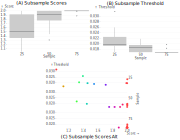
\includegraphics[width=0.5\textwidth]{./figures/subsampling.png}
	\caption{ (A) Box plot representing the AUTO-TUNE scores across ten random
		samples at 25\%, 50\%, and 75\% of the \citep{rhee_national_2019} dataset,
		showing a trend of increasing confidence in score estimates with denser
		sampling. (B) Box plot of the selected distance thresholds across the same
		random samples at 25\%, 50\%, and 75\% proportions, demonstrating improved
		consistency in threshold selection with increased sample size. (C)
		Scatterplot of the chosen thresholds (Y-axis) against their corresponding
		AUTO-TUNE scores (X-axis) for the three subsample proportions.
	}\label{fig:subsampling}
\end{figure}

\begin{figure}[h!]
	\centering
	\includegraphics[width=0.5\textwidth]{./figures/subsampling2.png}
	\caption{
		Figure A and B present the effects of subsampling on network structure using different thresholds. Figure A illustrates the proportion of nodes subsampled that remained clustered in both the original and the subsampled networks, with an observable increase in nodes captured as the threshold transitions from 1.5% to the optimized AUTO-TUNE threshold across subsampling levels (25%, 50%, and 75%). This pattern underscores the AUTO-TUNE scoring method's efficacy in preserving the network's structural integrity in subsampled datasets. Conversely, Figure B shows the proportion of nodes that were singletons in the original network and clustered in the subsampled networks. Despite varying subsampling rates and iterations, the impact of AUTO-TUNE's adaptive thresholding on clustering these singletons appears minimal, suggesting a negligible influence on the overall network structure.
	}\label{fig:subsampling2}
\end{figure}

\begin{figure}[h!]
	\centering
	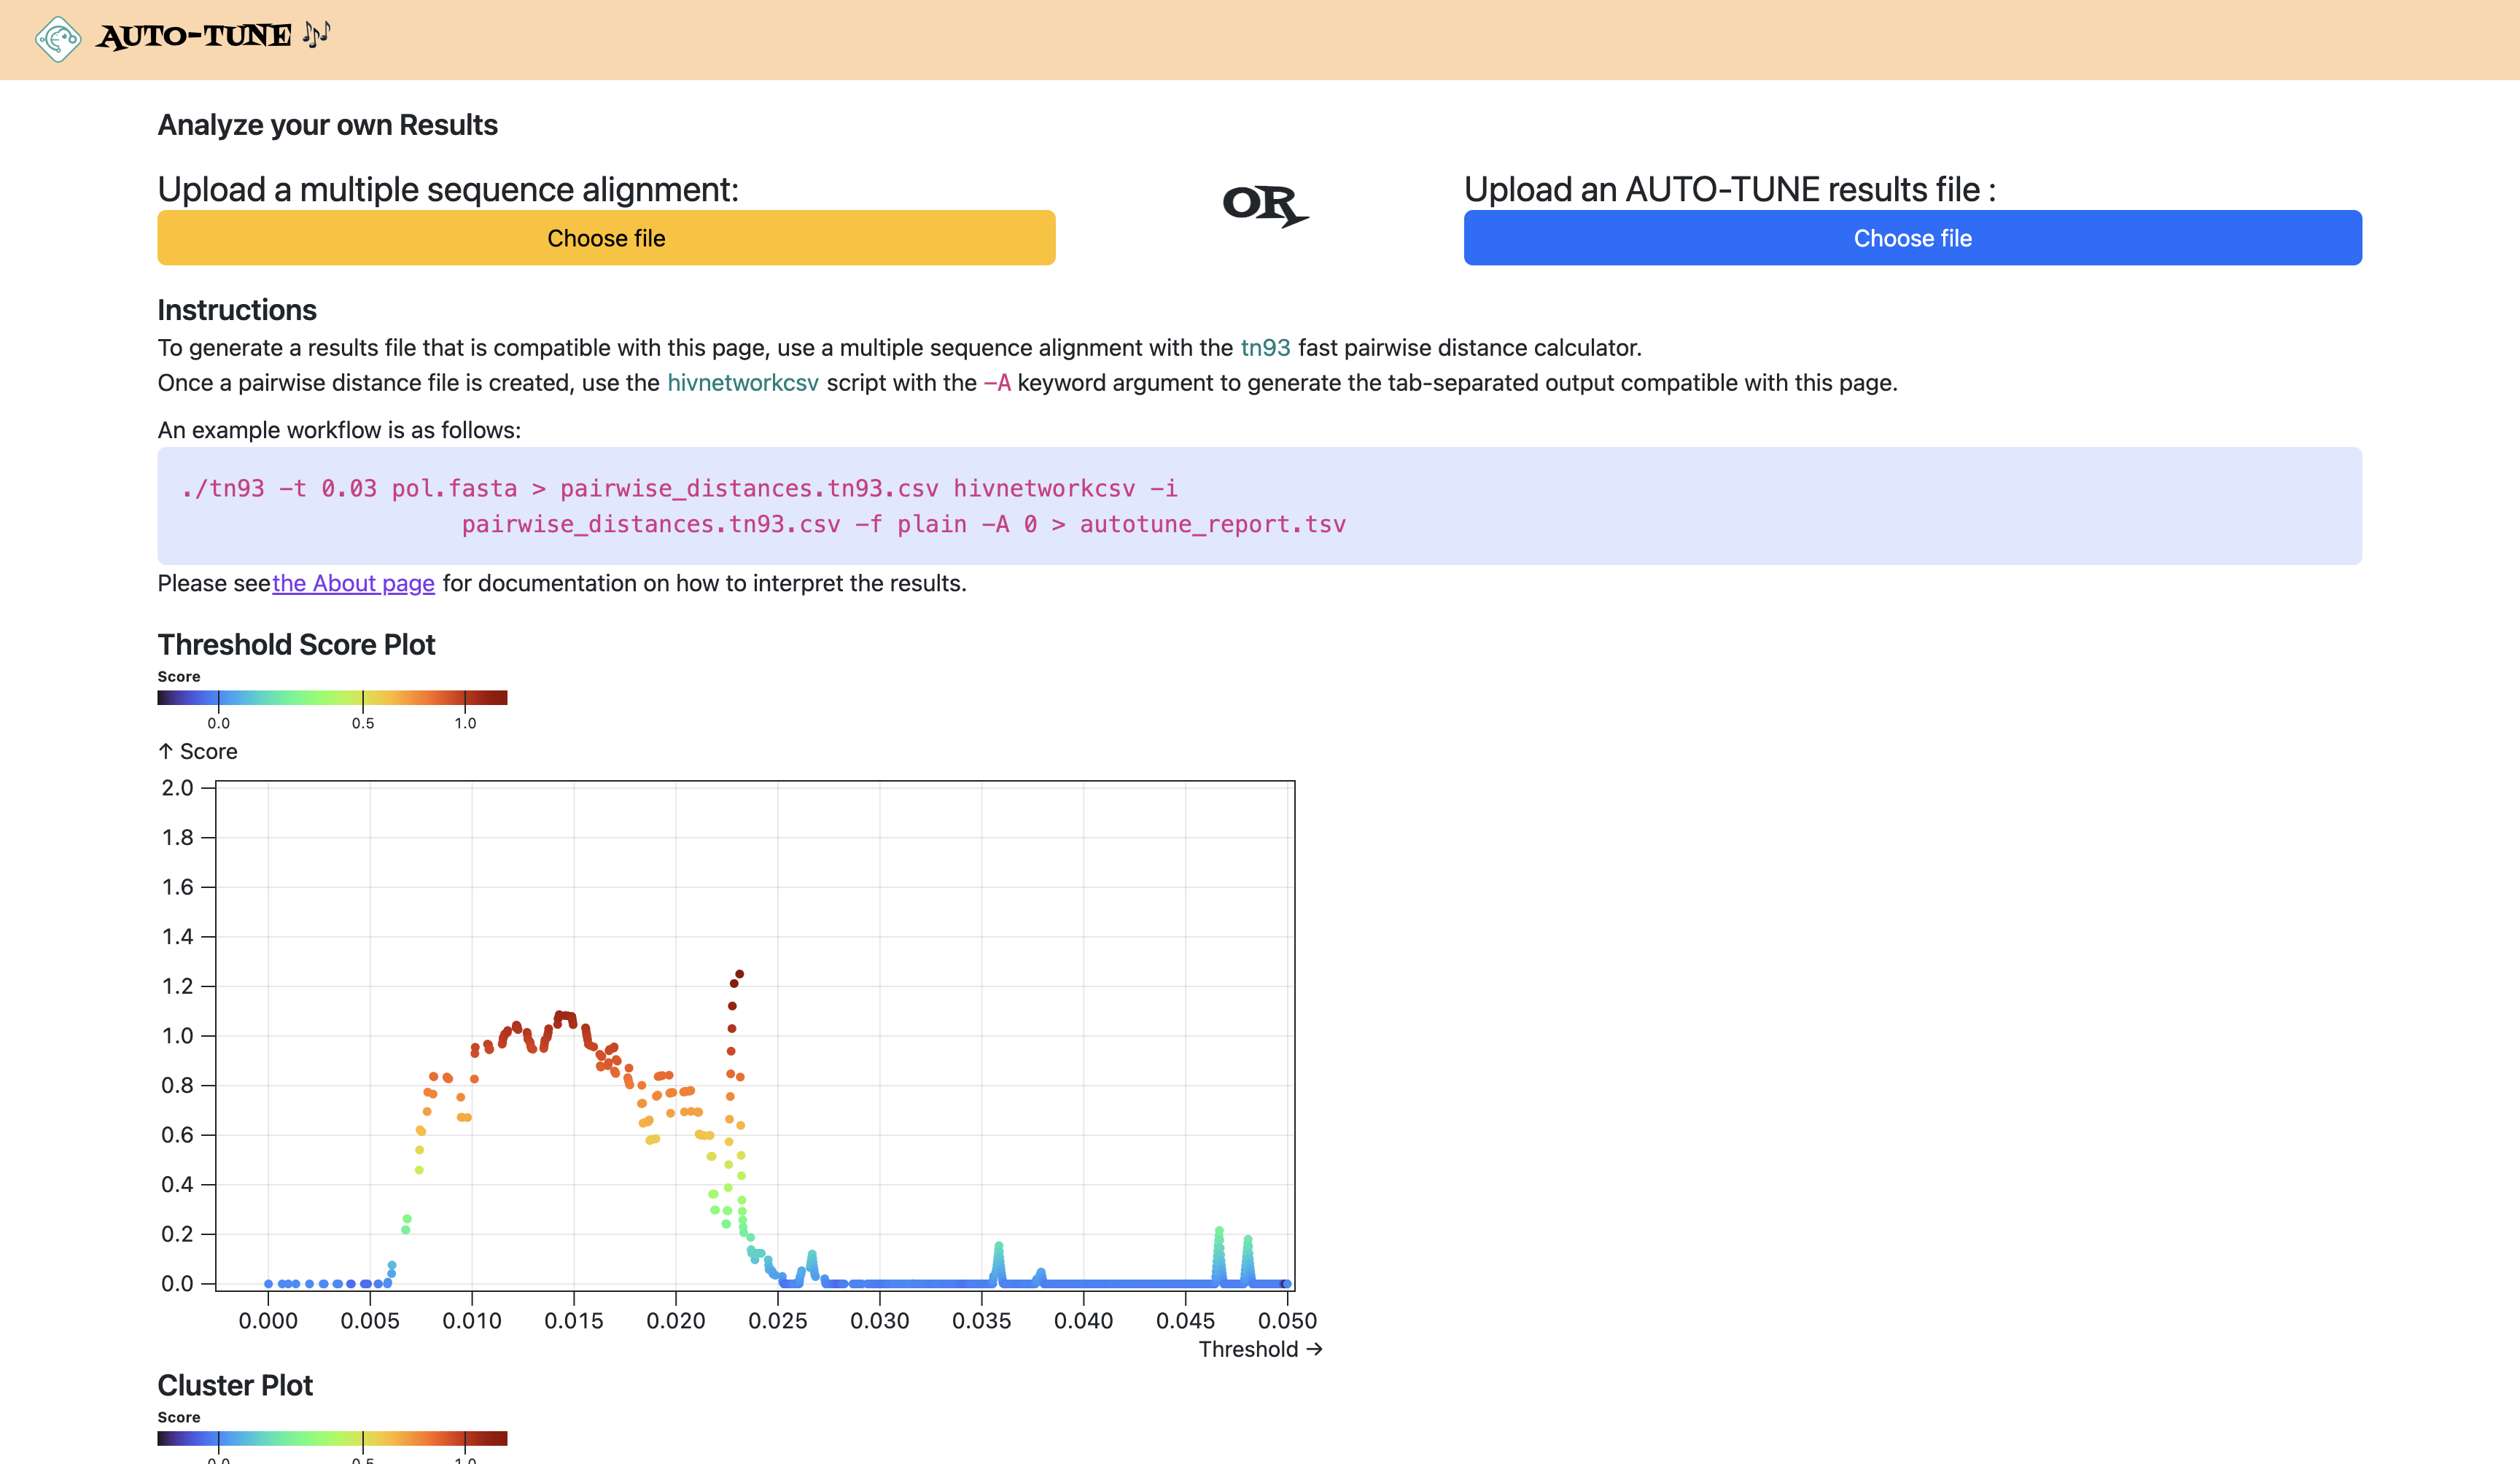
\includegraphics[width=0.5\textwidth]{./figures/webapp.png}
	\caption{ The user interface of the AUTO-TUNE web application
		(\url{http://autotune.datamonkey.org/analyze}). The platform provides a
		multi-faceted view of AUTO-TUNE's analysis, including a score plot that
		visualizes trends across different genetic distance thresholds. It also
		displays graphs of the number of clusters and the R1/R2 ratio—both key metrics
		in AUTO-TUNE's heuristic scoring system. These interactive visualizations aid
		researchers in making nuanced decisions for threshold selection, especially
		when multiple thresholds yield similar scores.
	}\label{fig:webapp}
\end{figure}

\begin{figure}[h!]
	\centering
	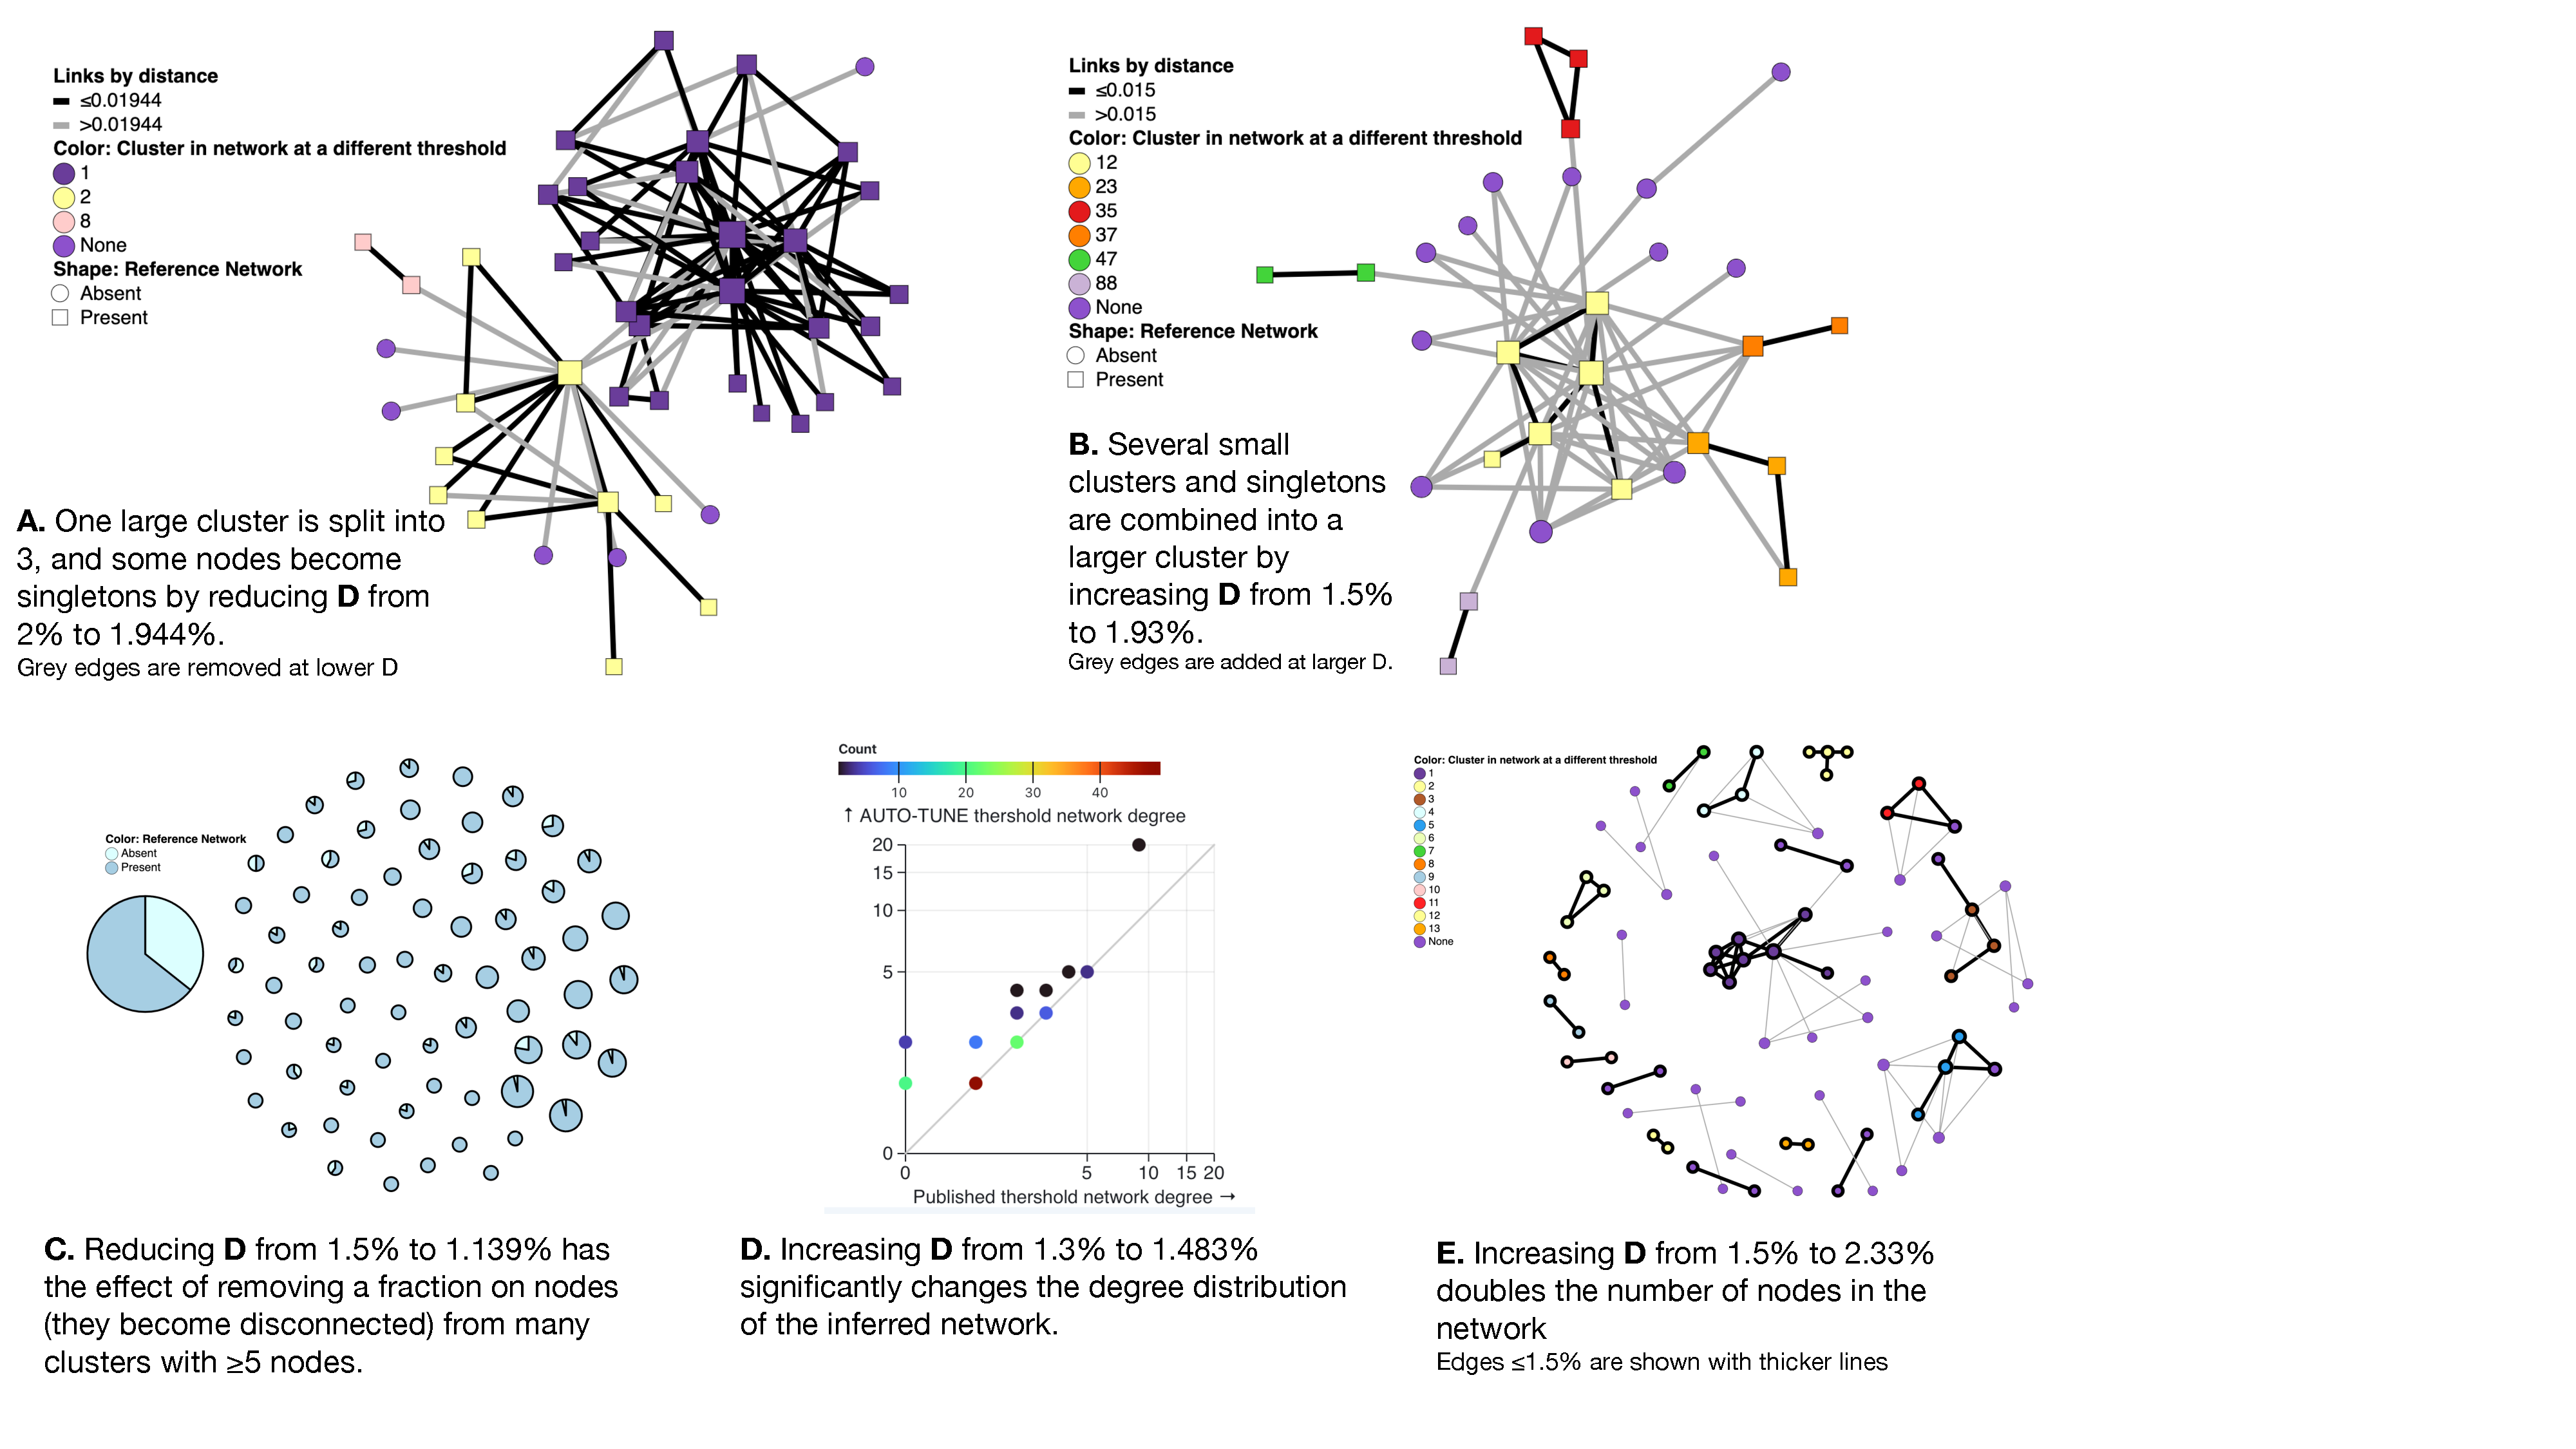
\includegraphics[width=1.\textwidth]{figures/examples.pdf}
	\vspace{0.01in}
	\caption{\textbf{Examples of AUTO-TUNE scores profiles.}
		(A). Lowering the genetic distance threshold removes some of the edges from the network (shown in grey) and disconnects a large cluster into color-coded smaller clusters; here "None" means that the node is not connected to anything at the lower threshold. (B). Raising the genetic distance threshold adds edges to the network (shown in grey) and connectes previously separte clusters into a larger component. (C). Each circle is a cluster in the larger threshold network, and with a proportion of nodes removed when the threshold is lowered. (D). Changes to the node degree distribution (colors represent the counts of nodes with the same degree). (E). A significant enlargement of a small network at a higher threshold, with grey edges only present at the larger threshold. }
	\label{fig:examples}
\end{figure}

\begin{figure}[h!]
	\centering
	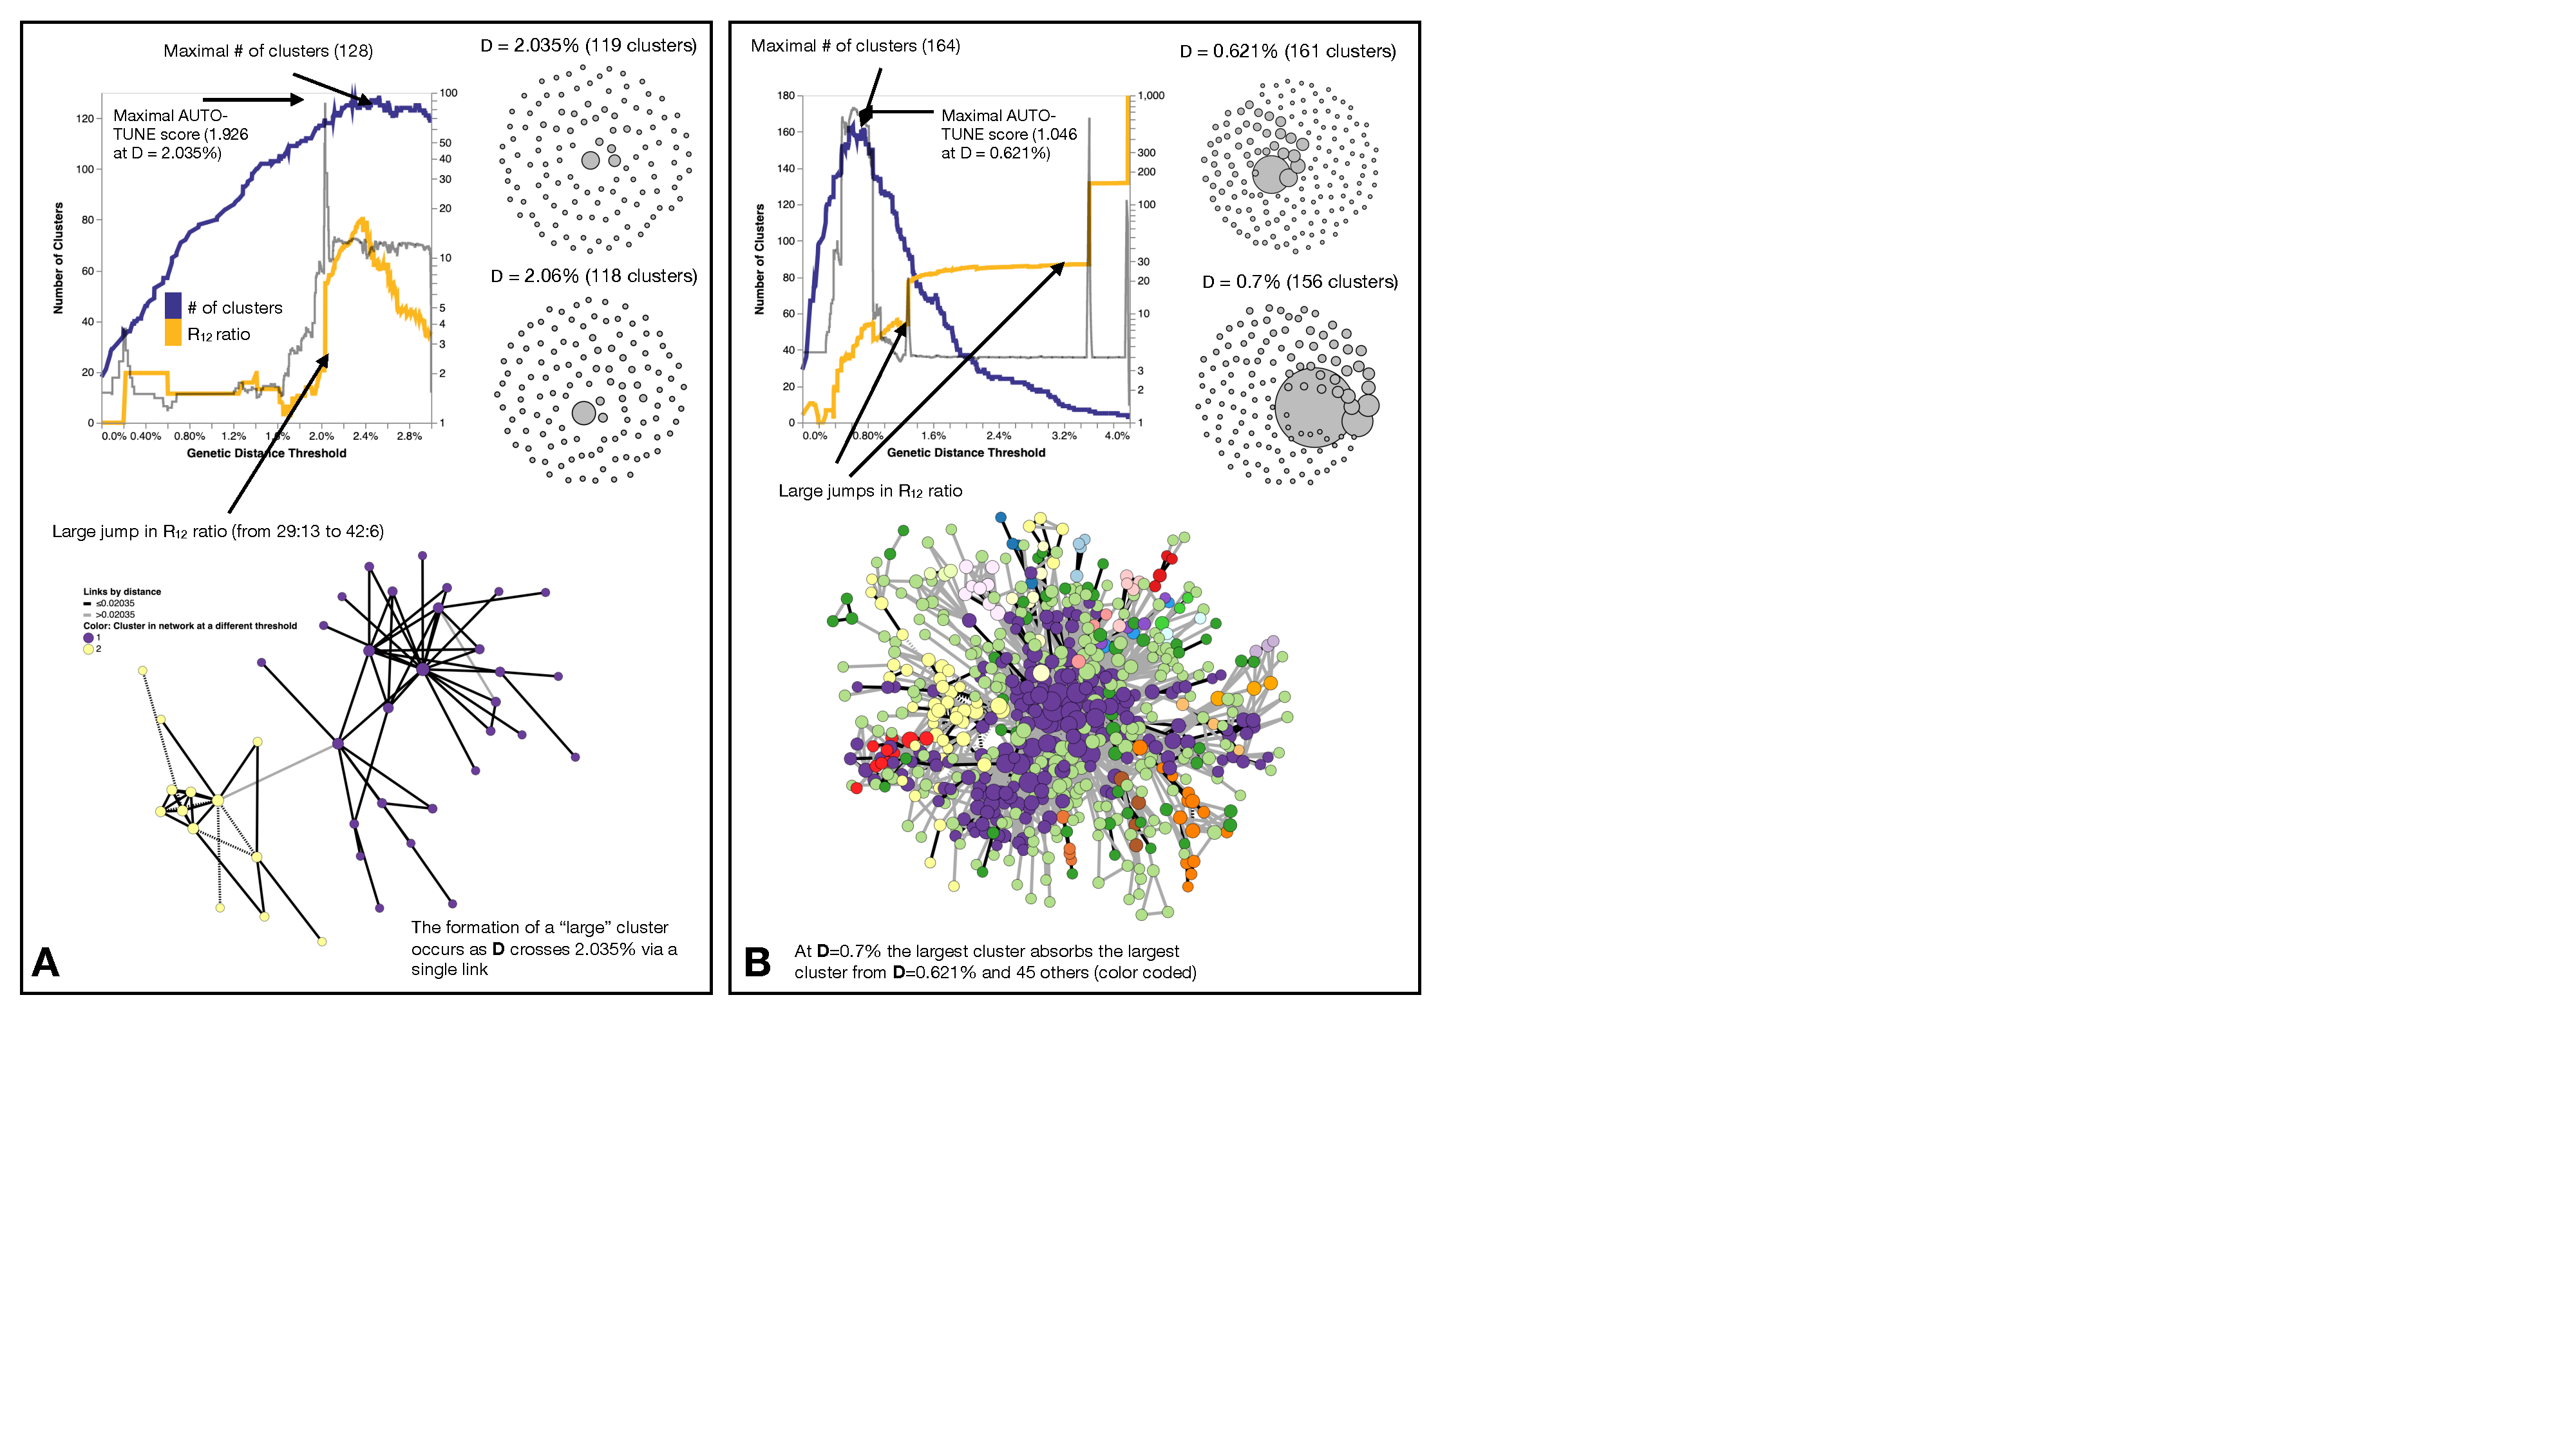
\includegraphics[width=1.\textwidth]{figures/cases.pdf}
	\vspace{0.01in}
	\caption{\textbf{Examples of how changing thresholds affects inferred networks.}
		(A). A high-scoring network \cite{bbosa_short_2020} has a distance threshold which achieves the number of clusters near the maximum, while also avoiding the formation of a large (weakly connected) cluster. (B). A low-scoring network \cite{liu_dynamics_2020} has a misalignment between the distance for which the maximum number of clusters is found, and where the big jumps in the cluster size ratio occur. Here, AUTO-TUNE effectively optimizes the number of clusters while preventing excessive growth of the largest cluster.}
	\label{fig:cases}
\end{figure}

\end{document}
